\insertdesignoverview{Chassis Stabilization Arms}
{Stabilize the chassis and set to numerous positions for various teleop objectives} % Goals of the mechanism
{arms_CAD.PNG}% CAD Image
{arms_build.PNG}% Build Image
{.25" Medium Density Fiberboard, Aluminum Shafting, PLA Plastic, Steel 1/2" Radial Bearings}% Materials ex. 0.25" MDF, Aluminum, etc
{Laser Cutting, 3D Printing, Lathe work, CNC Milling}% Manufacturing Processes ex. Laser Cut, 3D print, etc.


\interesting{Accomplishing chassis stabilization through innovative arms}{Innovate:55}
\interesting{}{Stabilize:1}

\subsection*{How it Works}
40:1 Torquenado motors actuate the arms using chain and sprocket with a 1:2 gear ratio. Each side features two 8" arms with skateboard wheels. Zeroed perpendicular to the chassis, the arms set to a natural stabilization position during autonomous, keeping Bullseye's floating chassis level as it drives. During crater scaling, the arms are programmed to actuate in accordance with the gyroscope, moving to keep the chassis balanced. Another arm set position readies the robot for shooting. Photointerruptors on each side ensure that the arms can find it's position during teleop in case of emergency.   

\subsection*{Modelling \& Simulation}
When designing the chassis stabilization arms, we established a body skeleton of the robot in PTC Creo, which was a basic sketch of the whole robot with set axes and coordinate systems. Then, we created motion skeletons for the individual arms. From there, we could build our parts around the skeleton, and attach them to the moving bodies. We could then simulate the movement within the motion skeleton. These skeletons not only helped us define the geometry and joints of the arms with several sketches, but they made major part modification simple since they're referenced to a base sketch, thus allowing us to change the arm design with ease. 

\begin{figure}[h!]
\centering
\begin{minipage}{.48\textwidth}
  \centering
  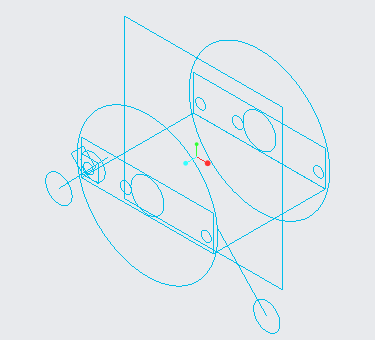
\includegraphics[width= .8\linewidth]{Design_Overview/Stabilization_Skeleton.PNG}
\end{minipage}%
\hfill
\begin{minipage}{.48\textwidth}
  \centering
  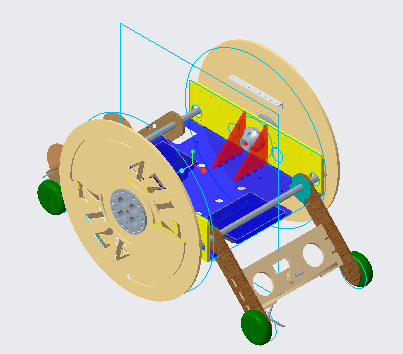
\includegraphics[width= .8\linewidth]{Design_Overview/Skel.PNG}
\end{minipage}
\end{figure}


\subsection*{Iterations}
Originally, our prototype chassis stabilization was done with primitive integration of the 4" Tetrix Omni Wheels and a short arm length. Not only did this haphazardous assembly fail to integrate well, with several wood spacers used to distance the bronze bushing to install the wheels, but the skinny wheel also made travel on the tiles much more difficult. We replaced the omnis with skateboard wheels, which made integration simple as it only required an 8mm screw with a washer and a nut. Another significant iteration we made was in regards to the arms' actuation. At first, we'd used HTD belts and 3D printed nylon pulleys with the same 1:2 ratio, yet we quickly recognized that the belt required incredible tension to run smoothly without skipping, which was so strong that it would twist the motor out of place, causing the belt to be loose yet again and causing it to skip. Realizing that a chain and sprocket system would be much more robust and less vulnerable to skipping, we replaced our pulleys with 16T to 32T VexPro sprockets with chain. 

\interesting{Design Iteration of the Stabilization Arms, Mark I to Mark V}{Design:4}

\begin{figure}[h!]
\centering
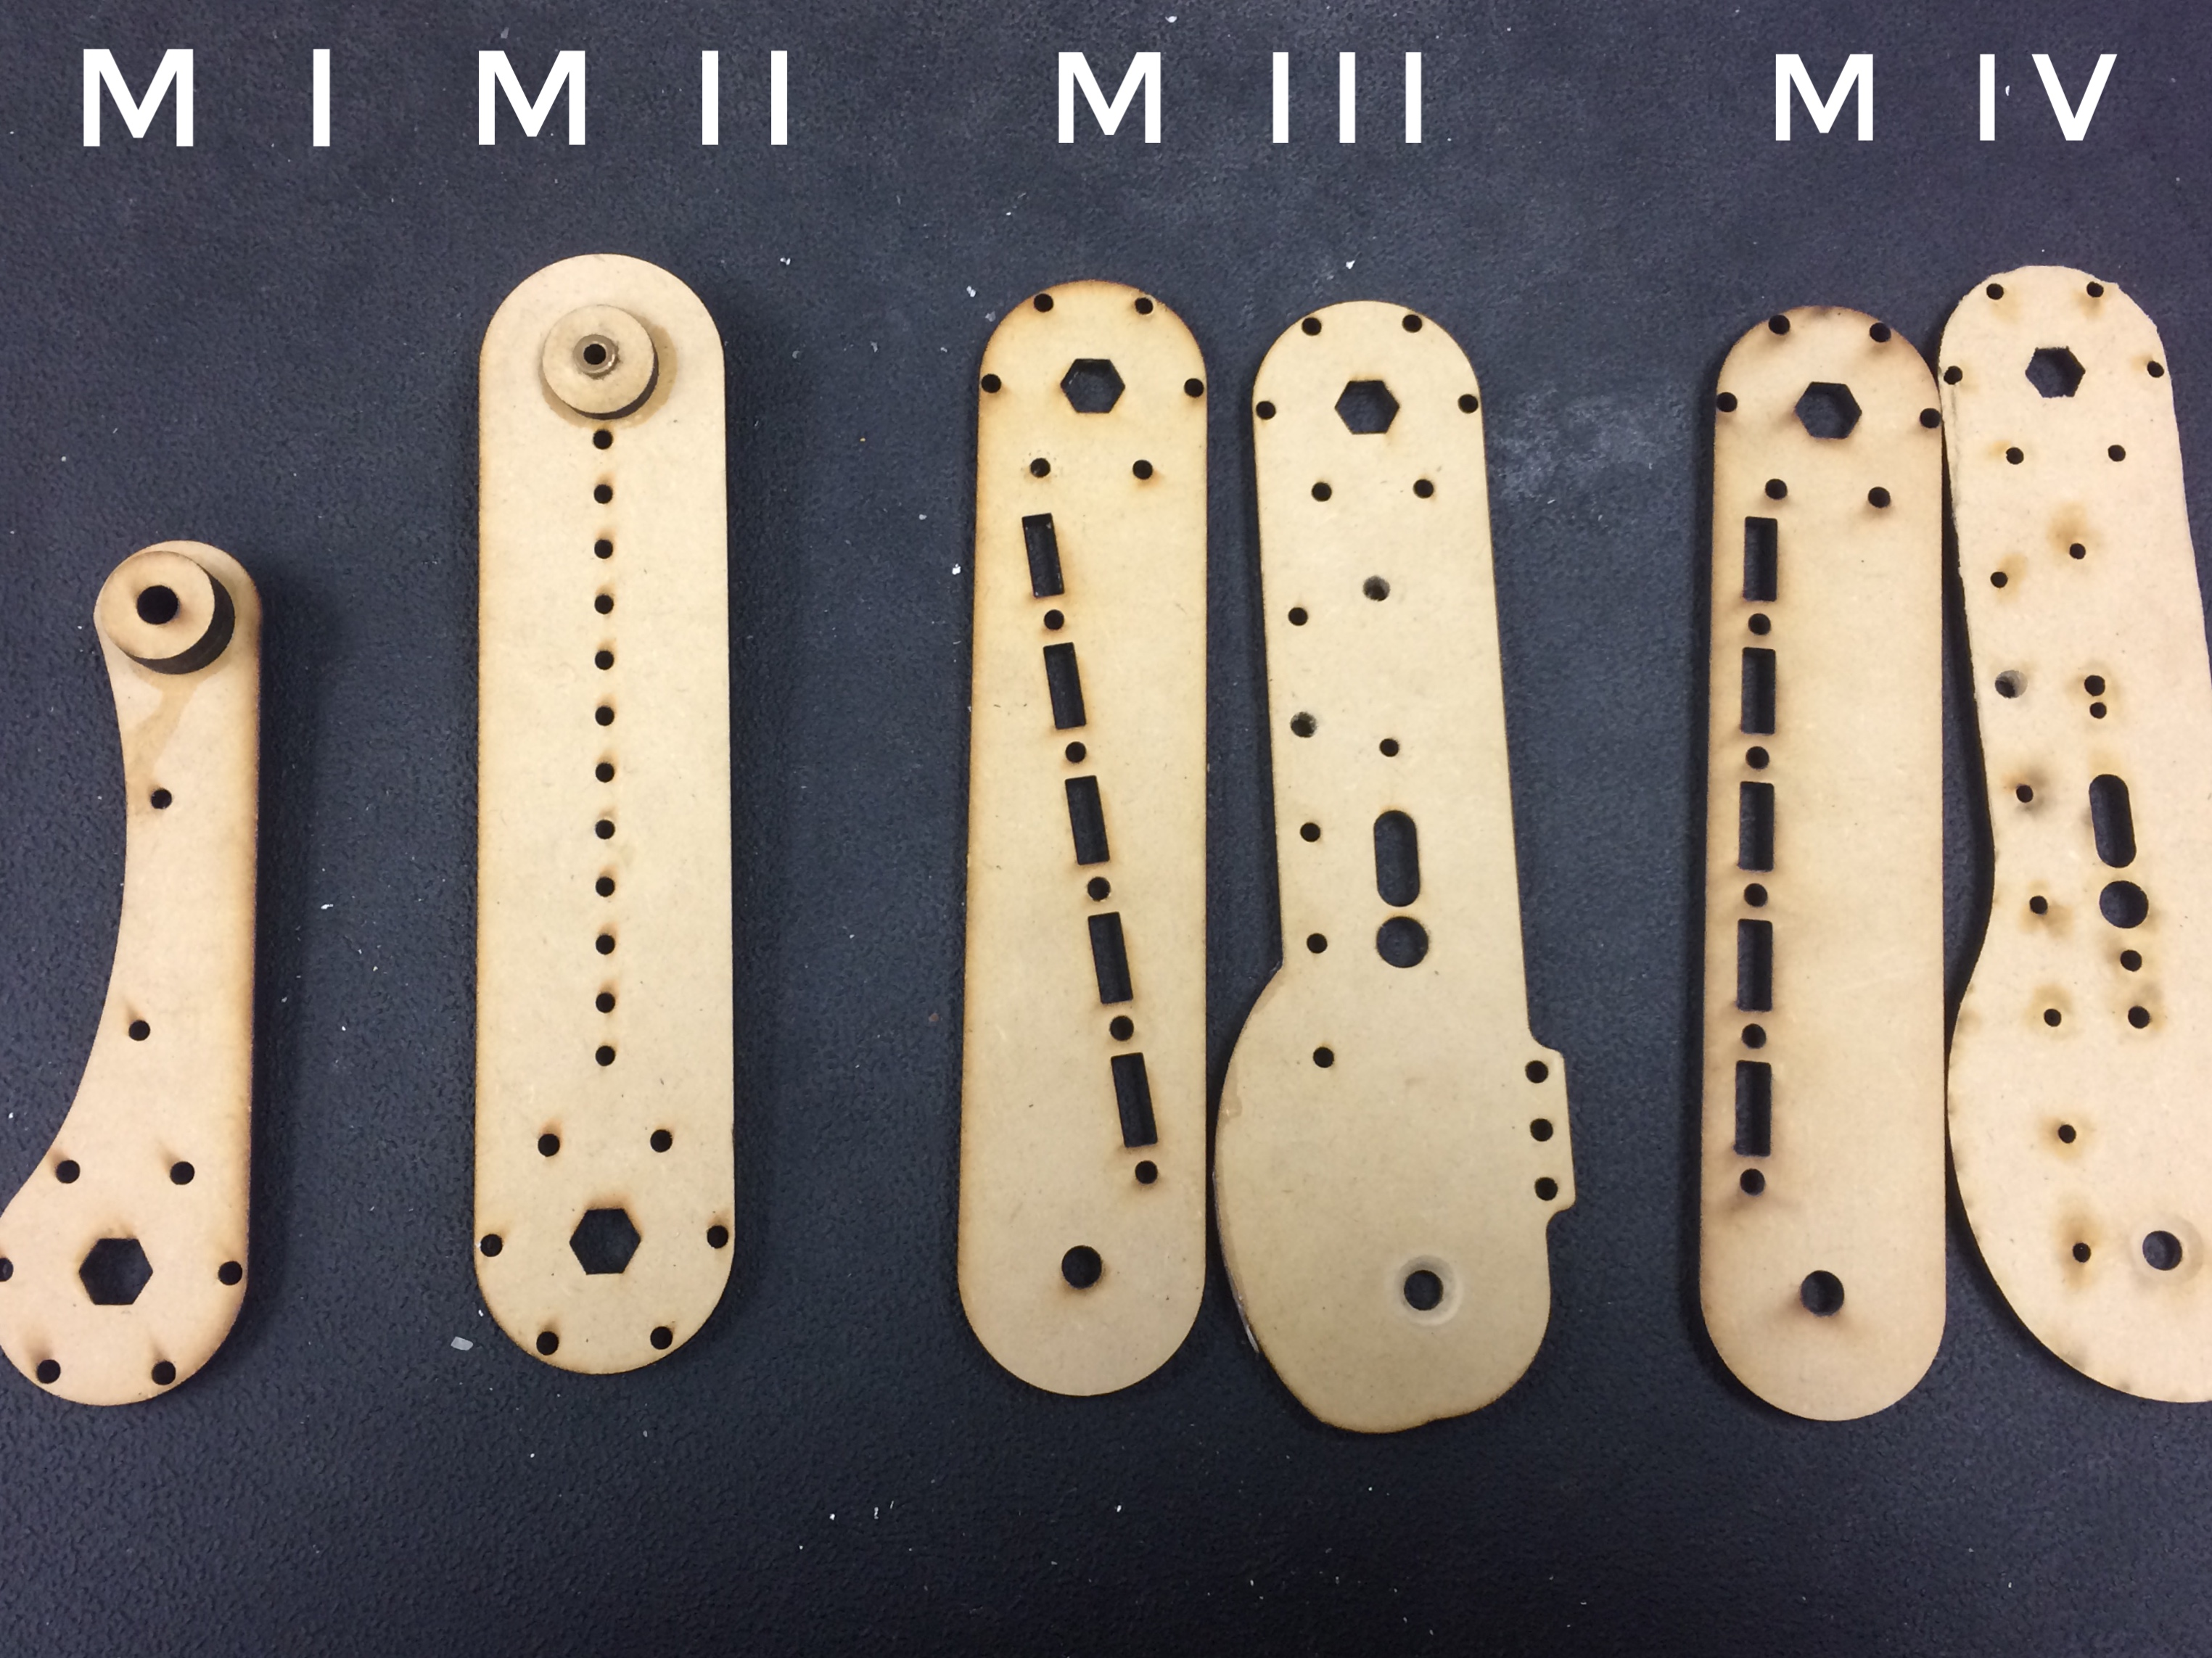
\includegraphics[width=.8\linewidth]{Design_Overview/Iteration.jpg}
\caption{Design Iteration of the Stabilization Arms, Mark I to IV}
\label{fig:iteration}
\end{figure}

\begin{figure}[h!]
\centering
\begin{minipage}{.32\textwidth}
  \centering
  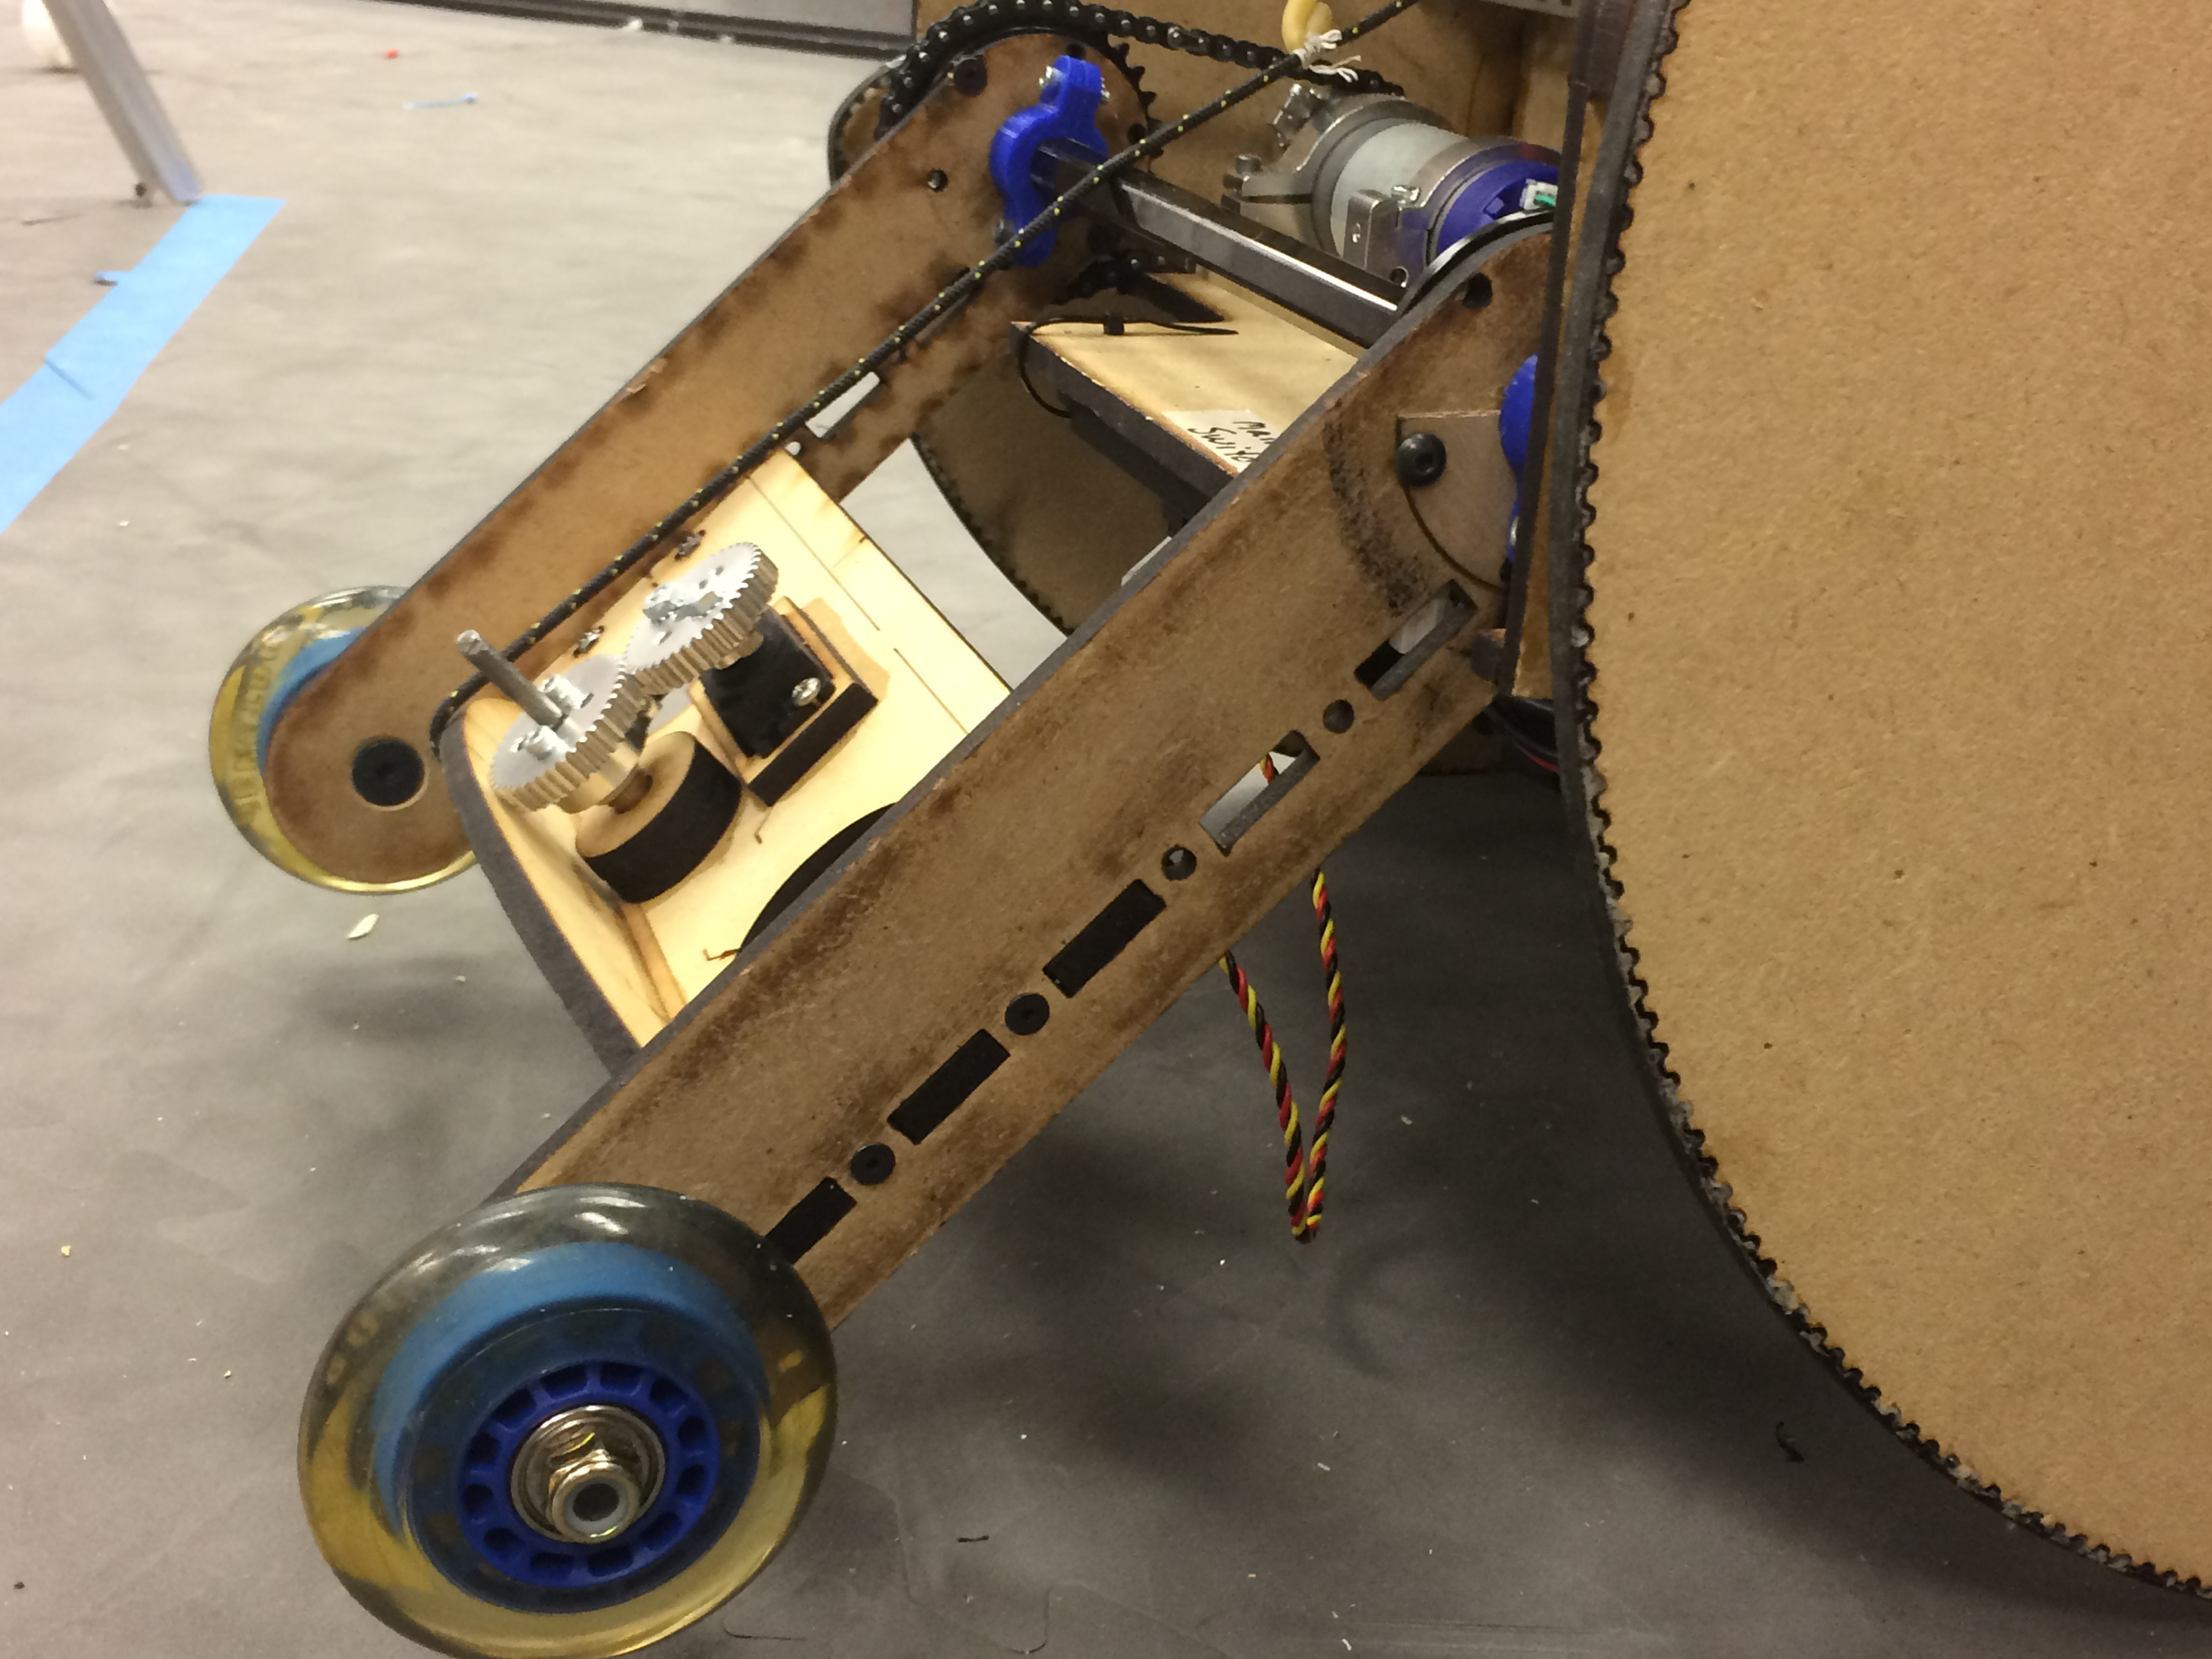
\includegraphics[width= .9\linewidth]{Design_Overview/front_arm.JPG}
\end{minipage}%
\hfill
\begin{minipage}{.32\textwidth}
  \centering
  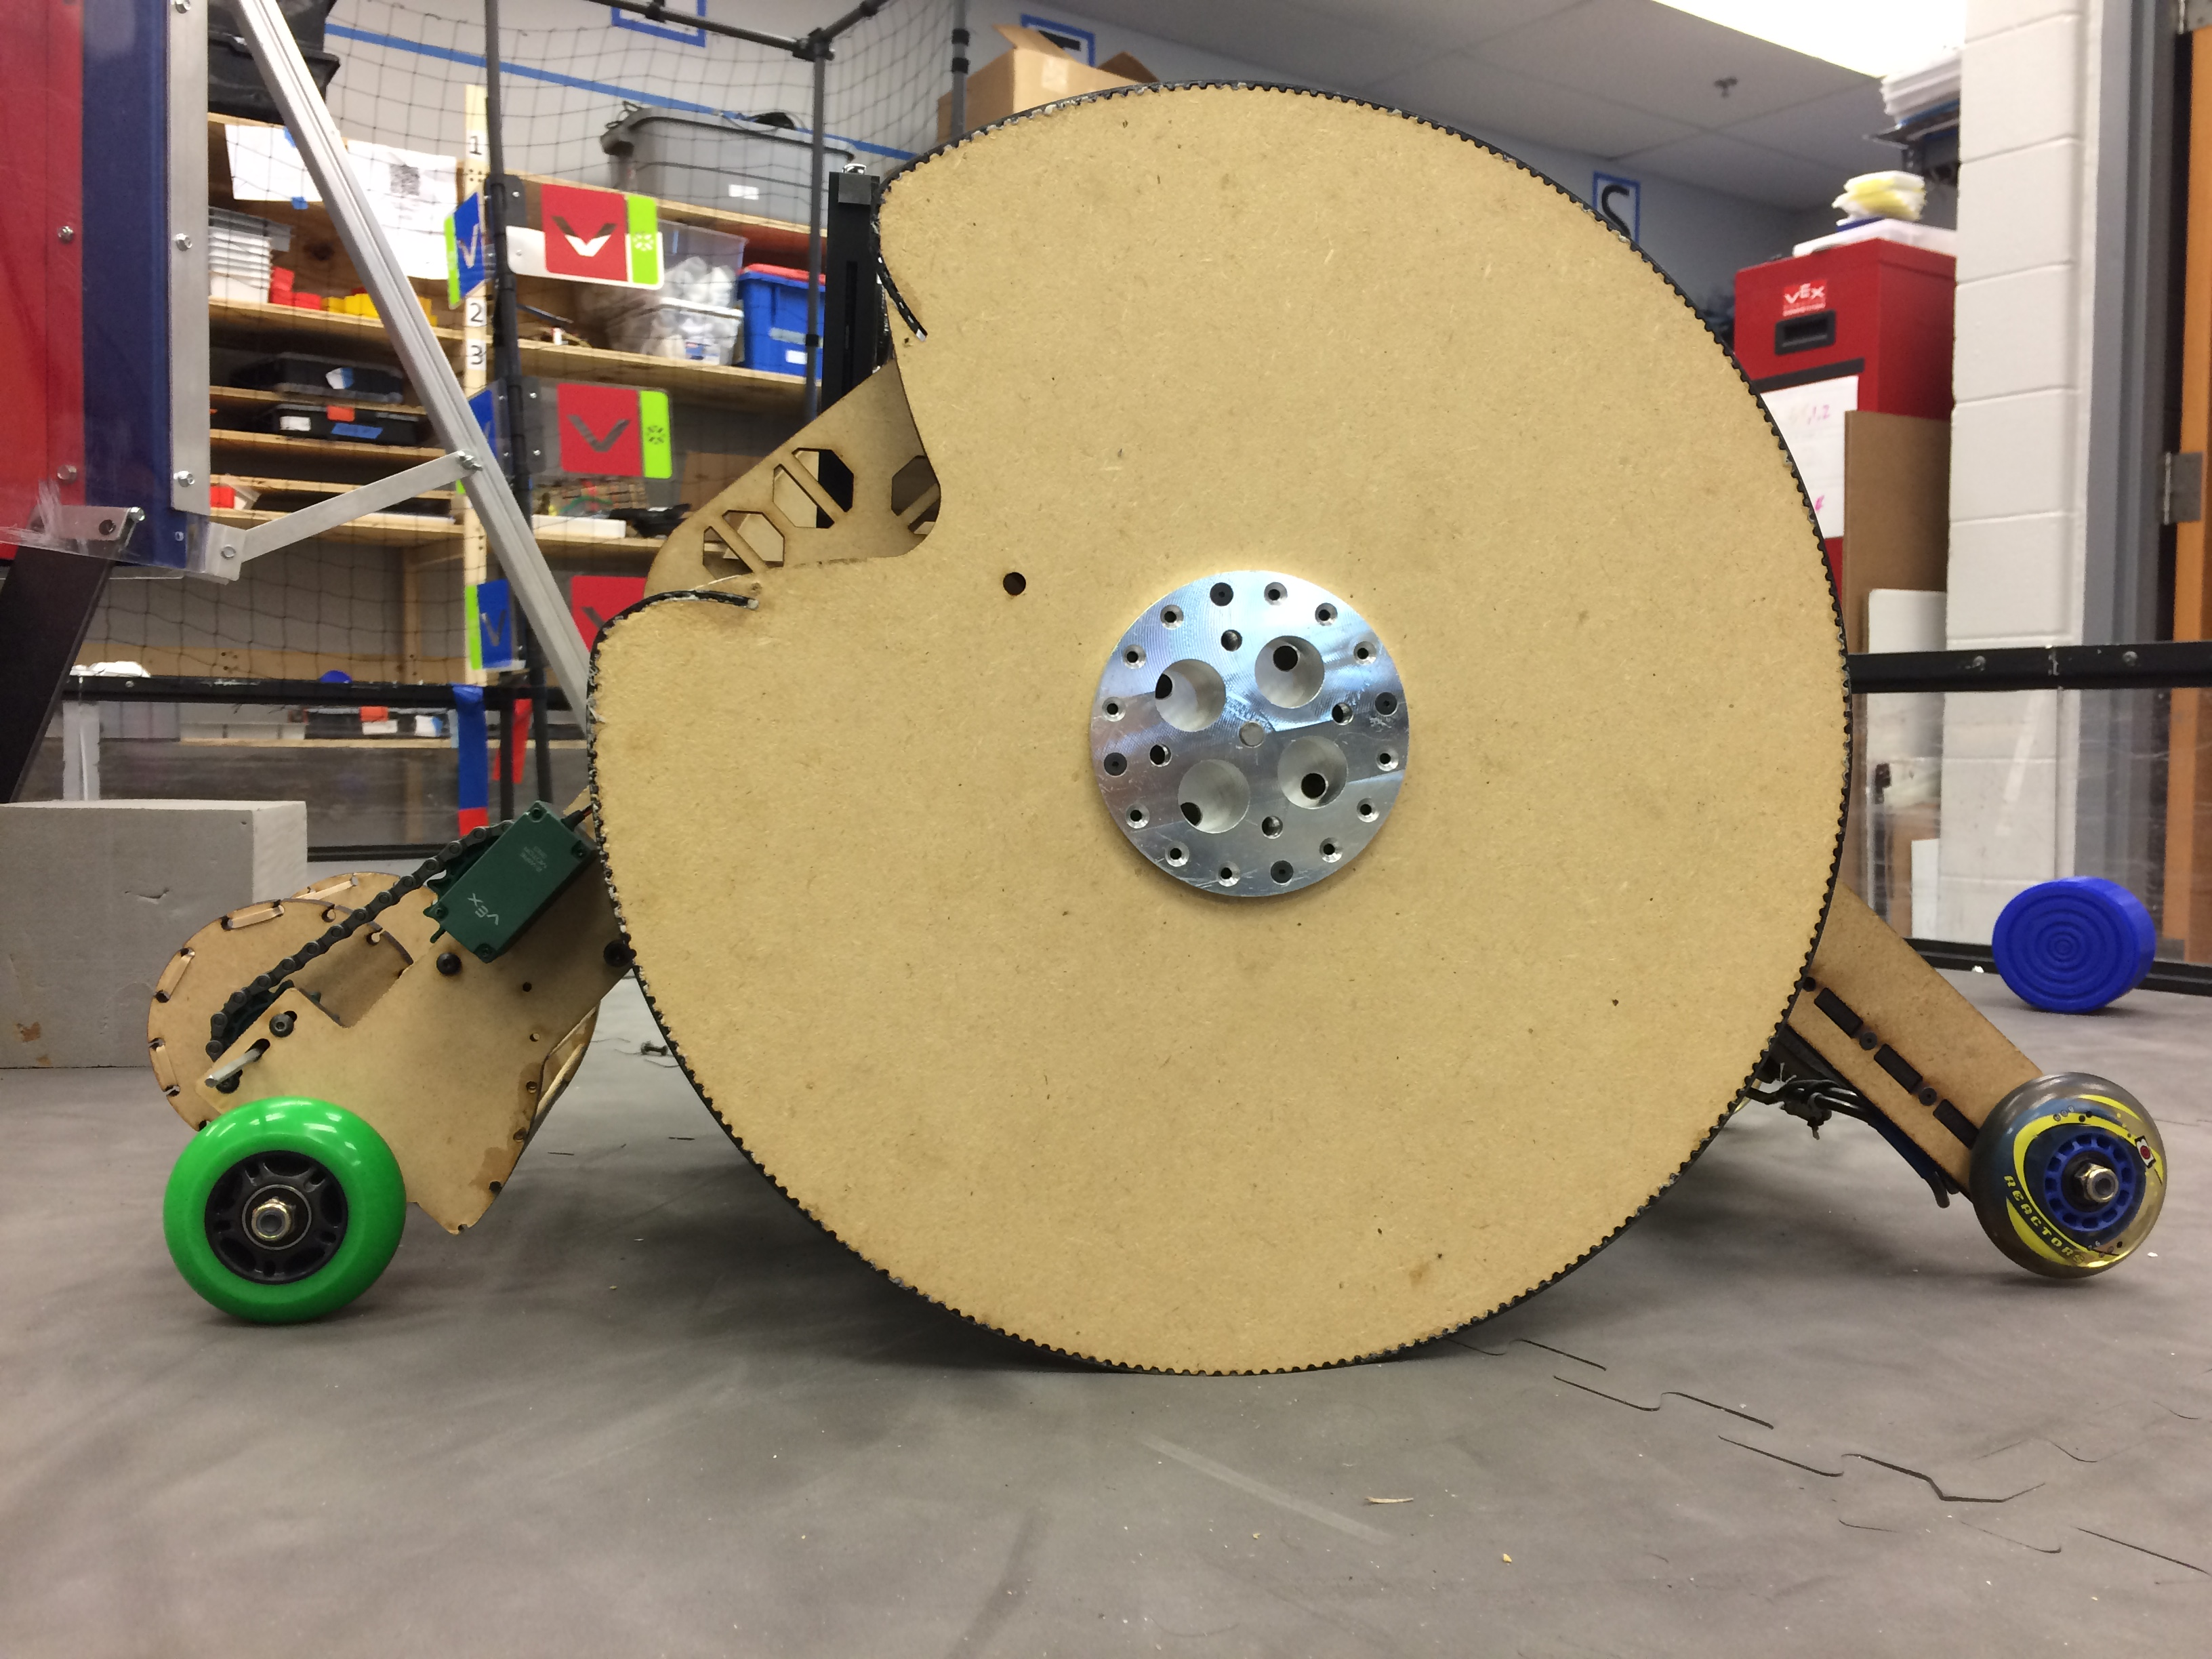
\includegraphics[width= .9\linewidth]{Design_Overview/both_arms.JPG}
	\caption{Final Stabilization Arms, Mark V}
	\label{fig:Triple_Arm_IMG}
\end{minipage}%
	\hfill
\begin{minipage}{.32\textwidth}
  \centering
  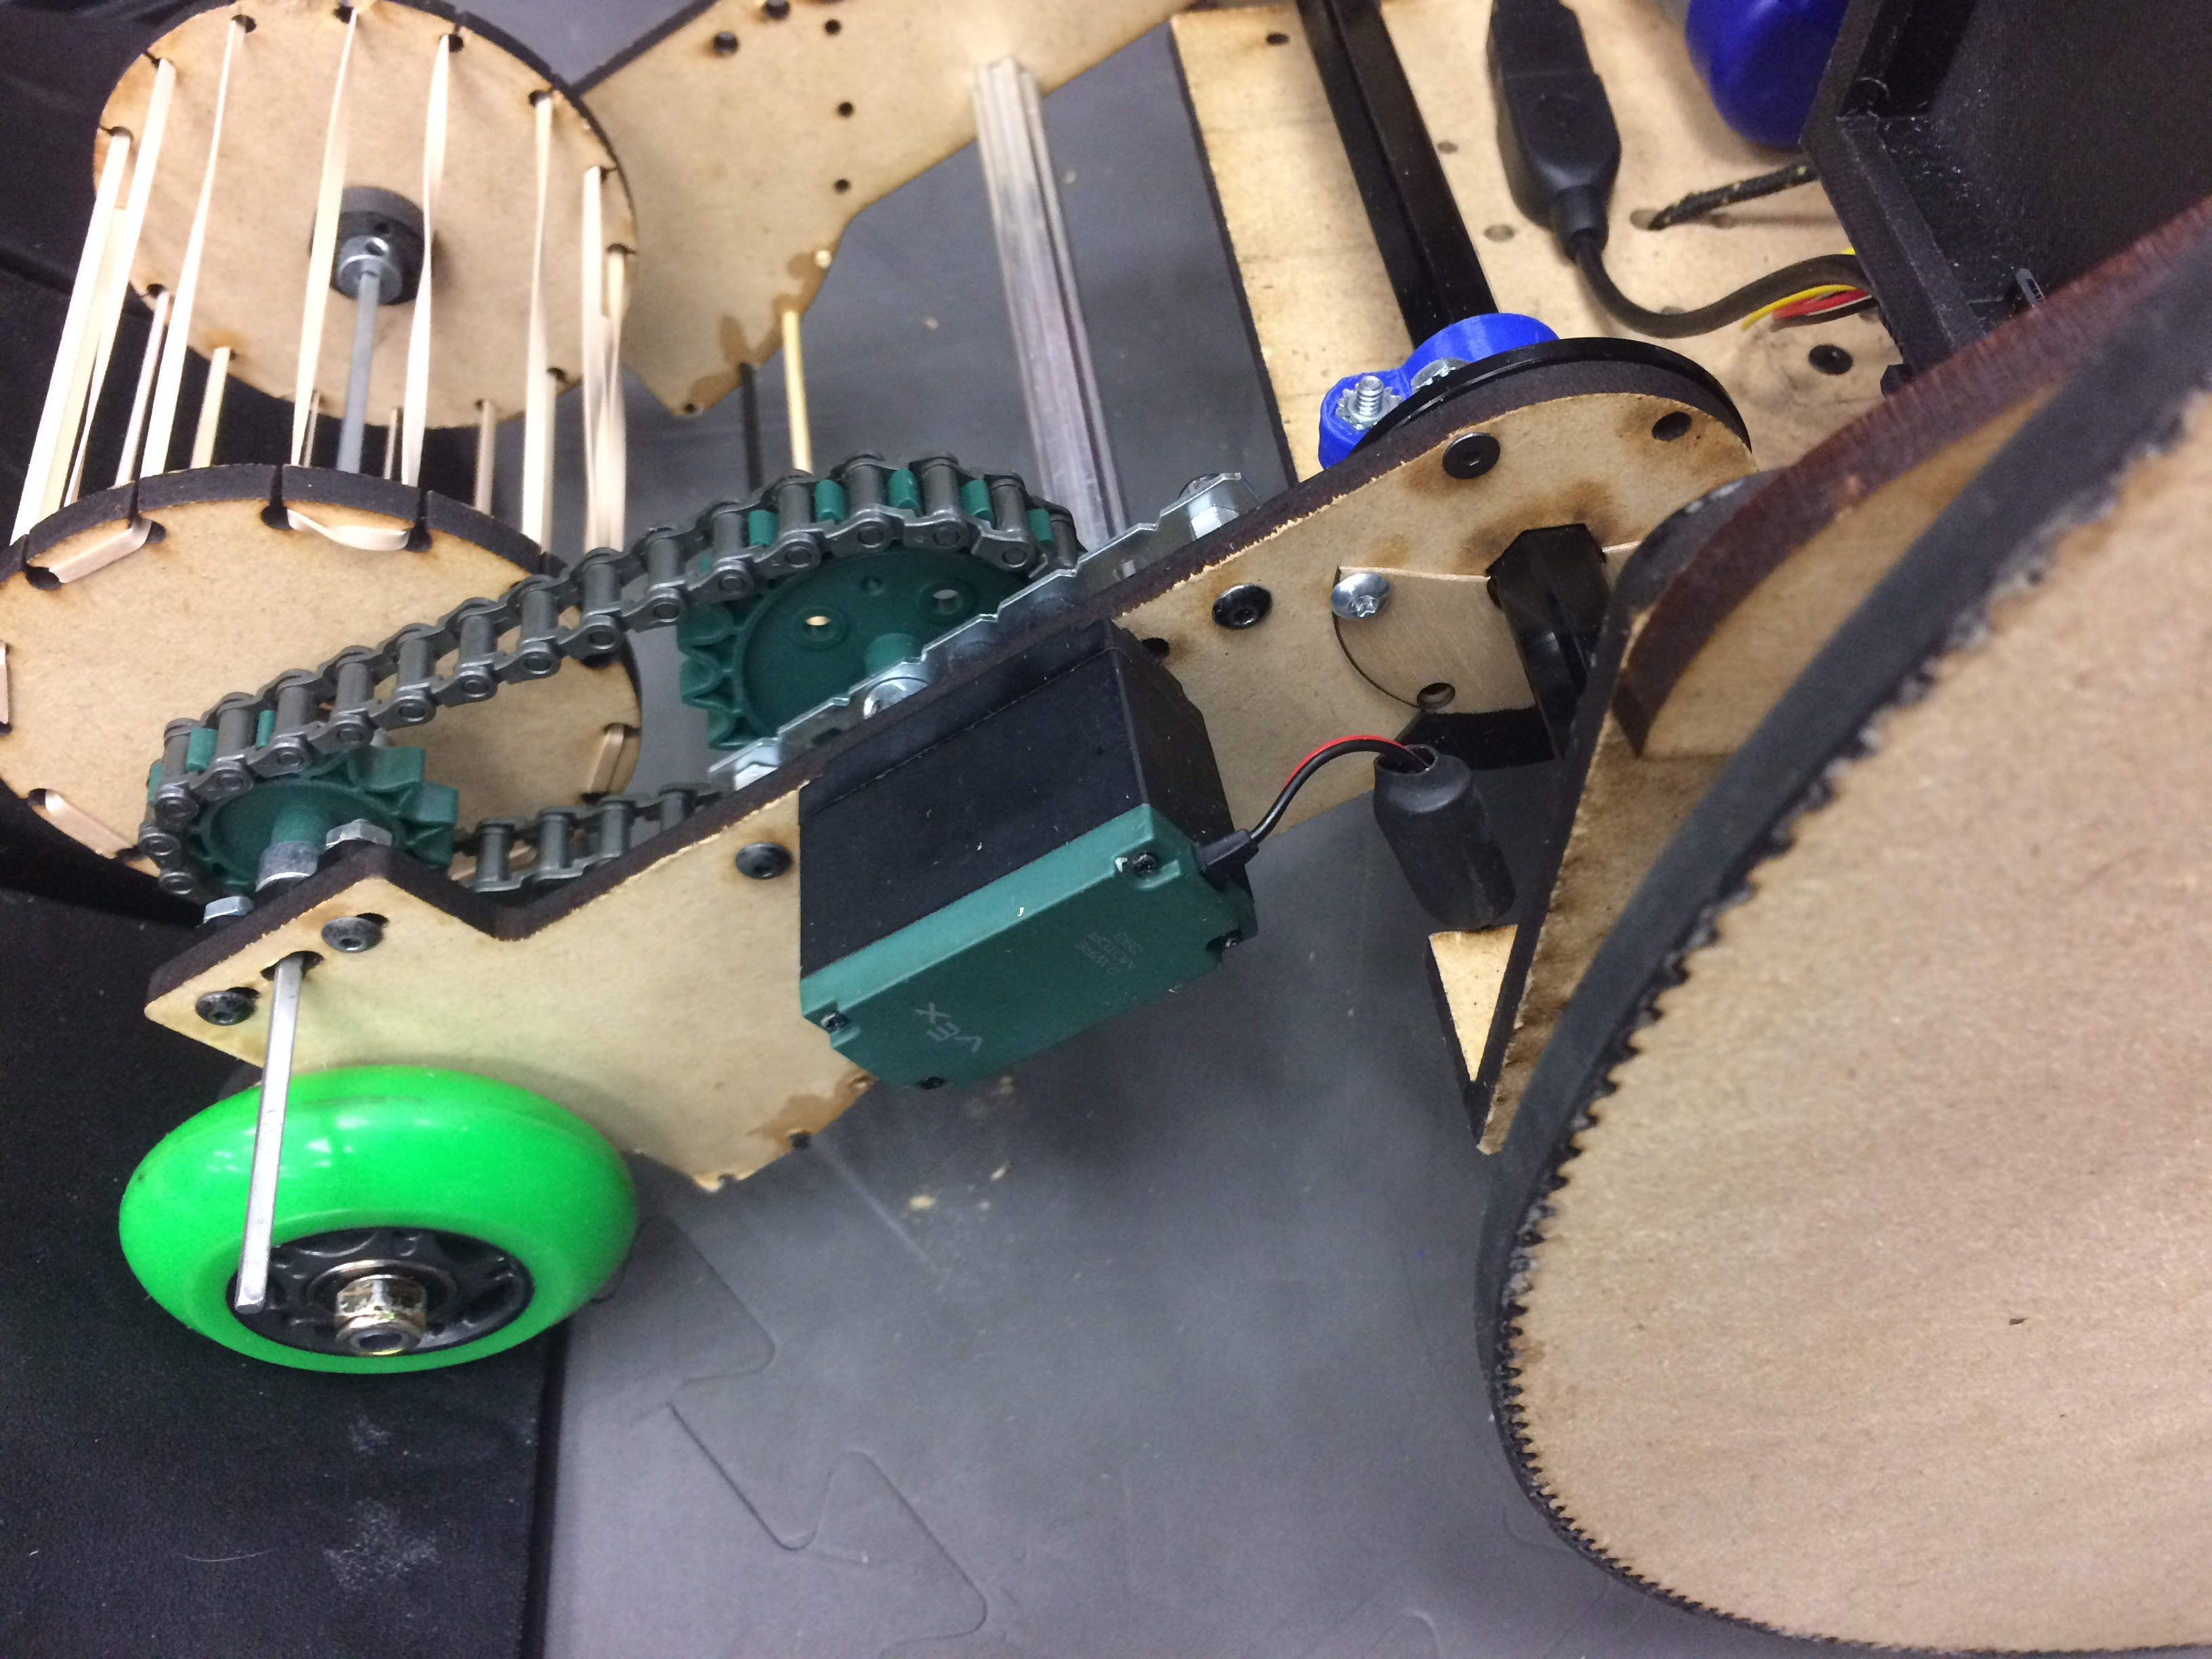
\includegraphics[width= .9\linewidth]{Design_Overview/rear_arm.JPG}
\end{minipage}
\end{figure}

\subsection*{Sensors and Control}
Two photointerruptors, one on each side, are used for emergency recalibration of the arms at their natural position. Two laser cut wooden flanges on each arm break the light beam of the photointerruptor, setting a known position for the arm. However, understanding that the encoders aren't perfect, and given the backlash of the chain, we understood that we had to come back up and return slower in order to calibrate at exactly the right position for driving smoothly. In addition, we use the internal PID on the REV Expansion Hub for stabilization, and utilize preestablished angles for various telemetry operations, such as intaking minerals, shooting into the lander, or hanging on the latch. For determining level driving angles for the arms, our physics division determined a formula to calculate the angle at which one arm would have to be in relation to the other. 

%\begin{figure}[h!]
%\centering
%\begin{minipage}{.48\textwidth}
%  \centering
%  \includegraphics[width= .8\linewidth, angle=-90]{Meetings/January/01-21-19/interrupter.png}
%\end{minipage}%
%\hfill
%\begin{minipage}{.48\textwidth}
 % \centering
%  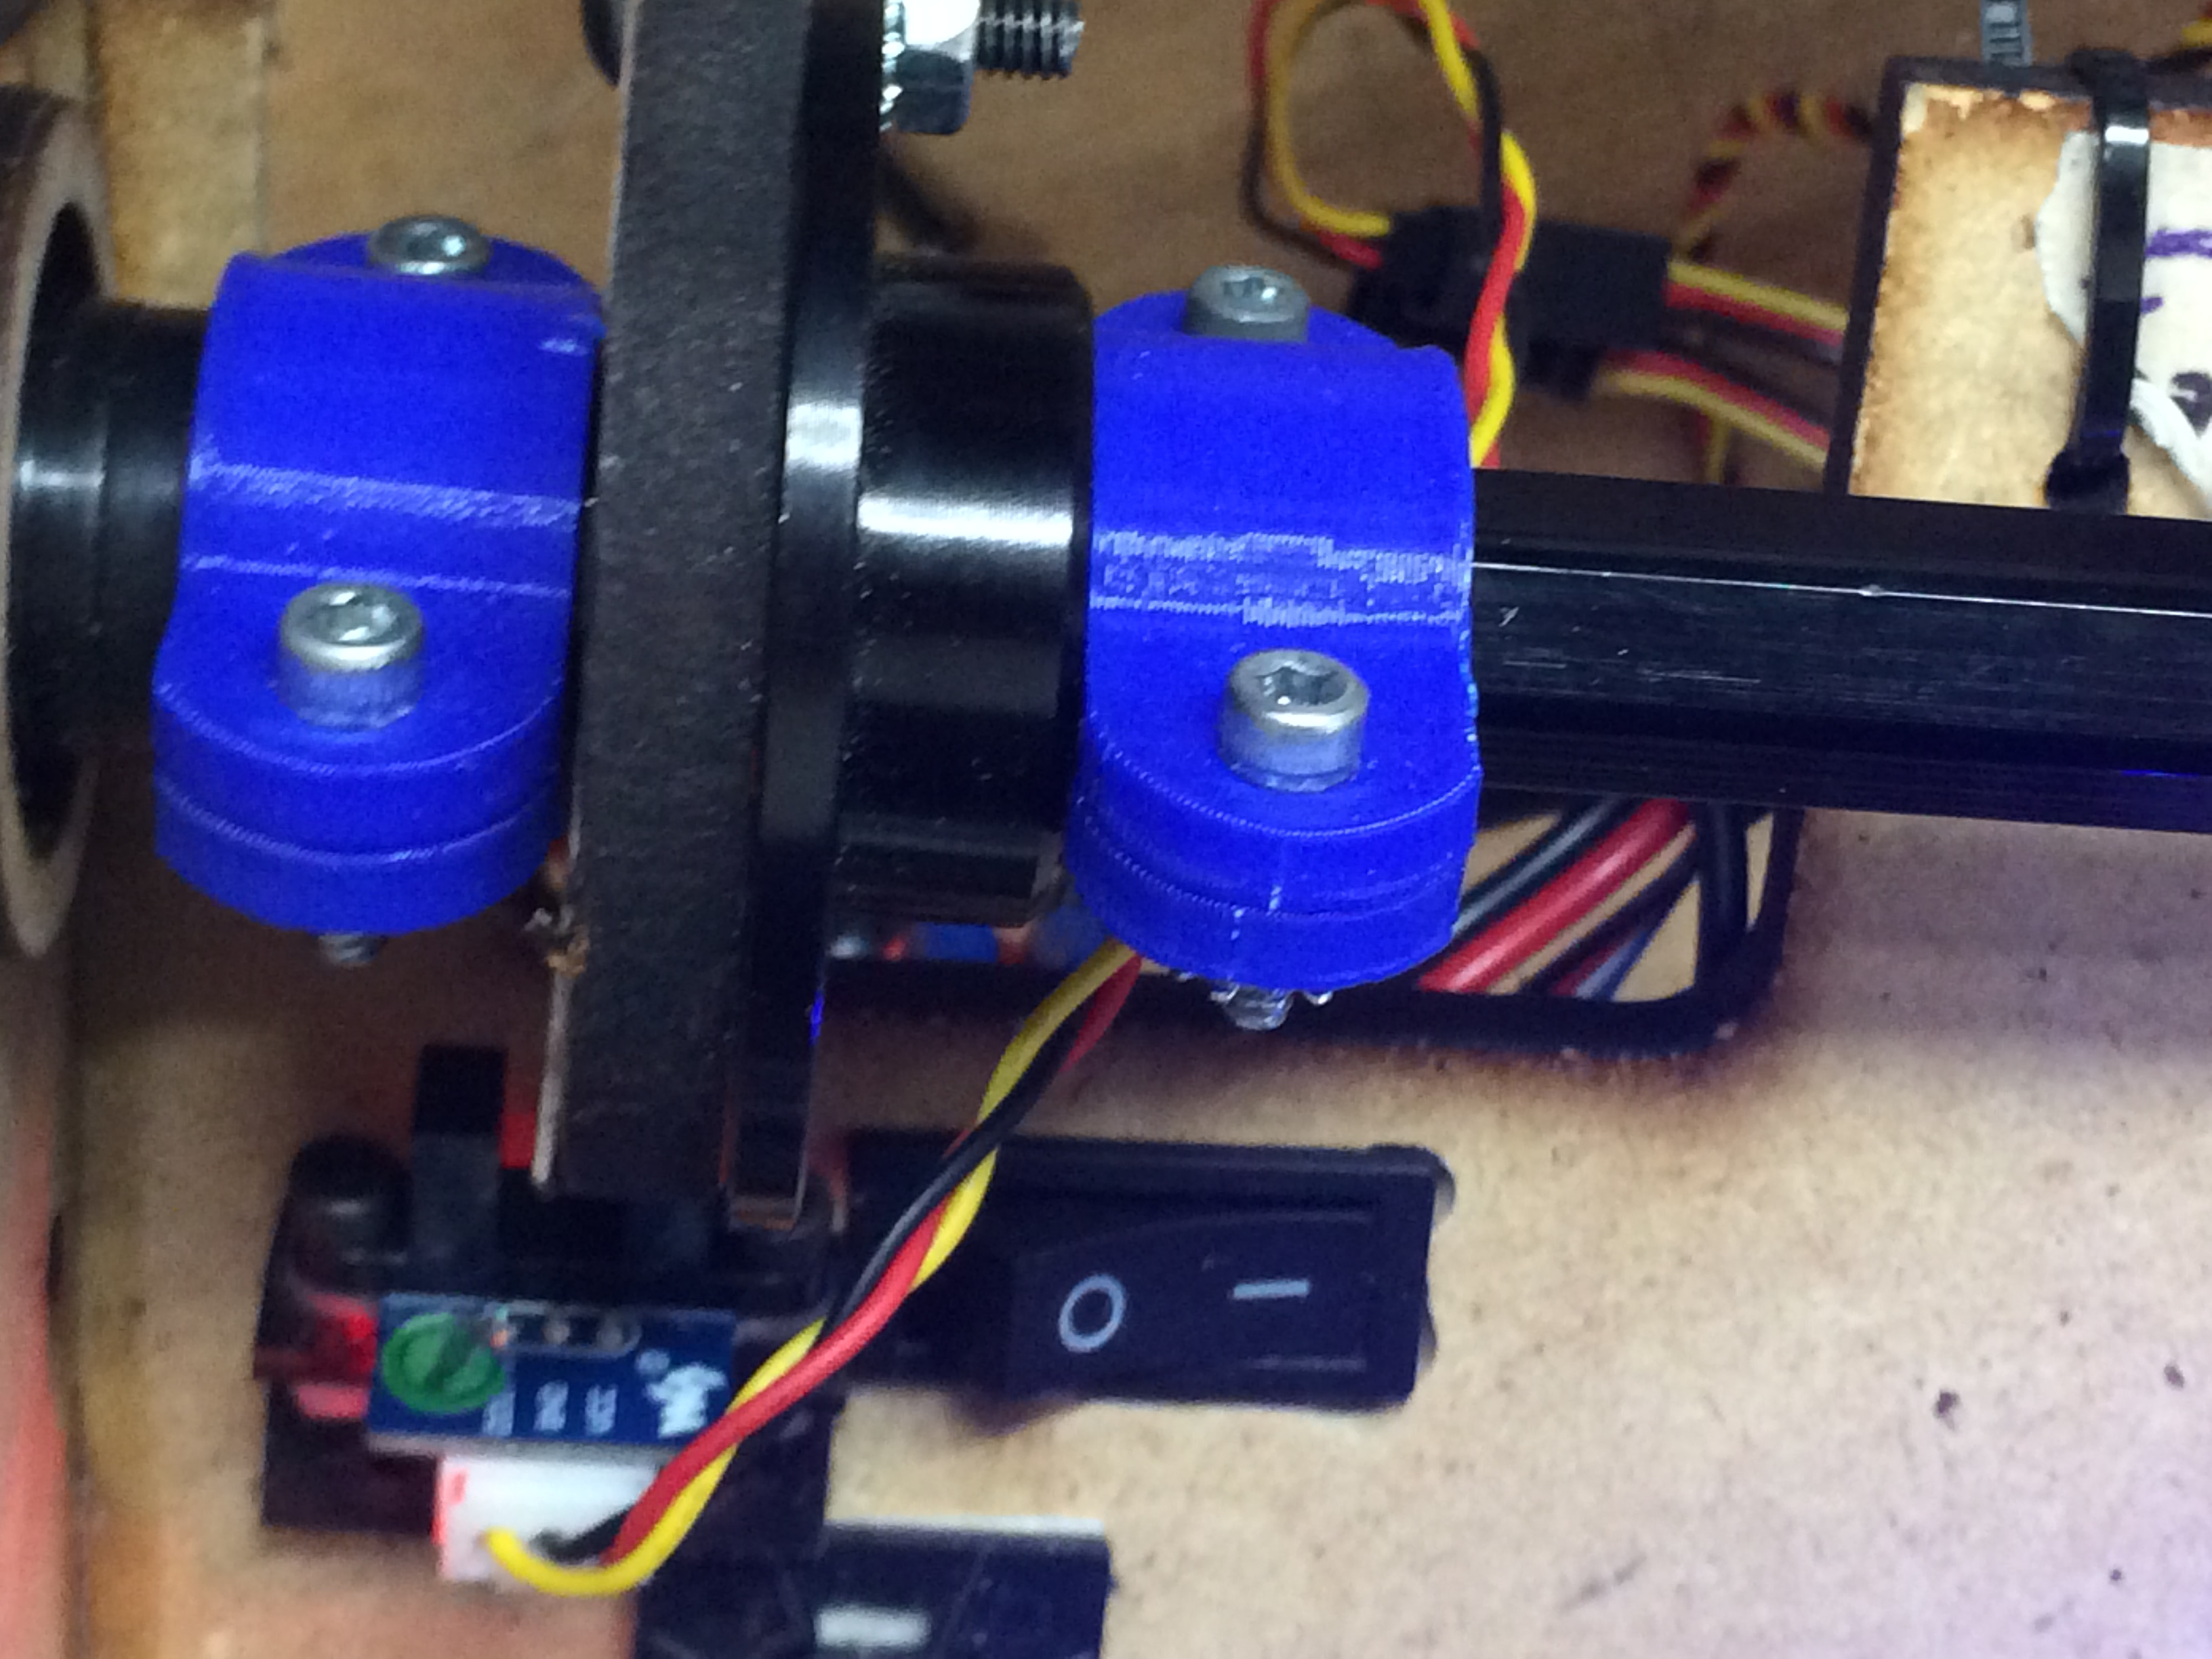
\includegraphics[width= .75\linewidth, angle=-90]{Design_Overview/photo_int_real.JPG}
%\end{minipage}
%\end{figure}

\vskip 0.35in
\textbf{Different Arm Preset Positions:}
\textit{Various Preset Positions for the Stabilizing Arms}

\interesting{Various Preset Positions for the Arms}{control:3}

\begin{figure}[h!]
\centering
\begin{minipage}{.32\textwidth}
  \centering
  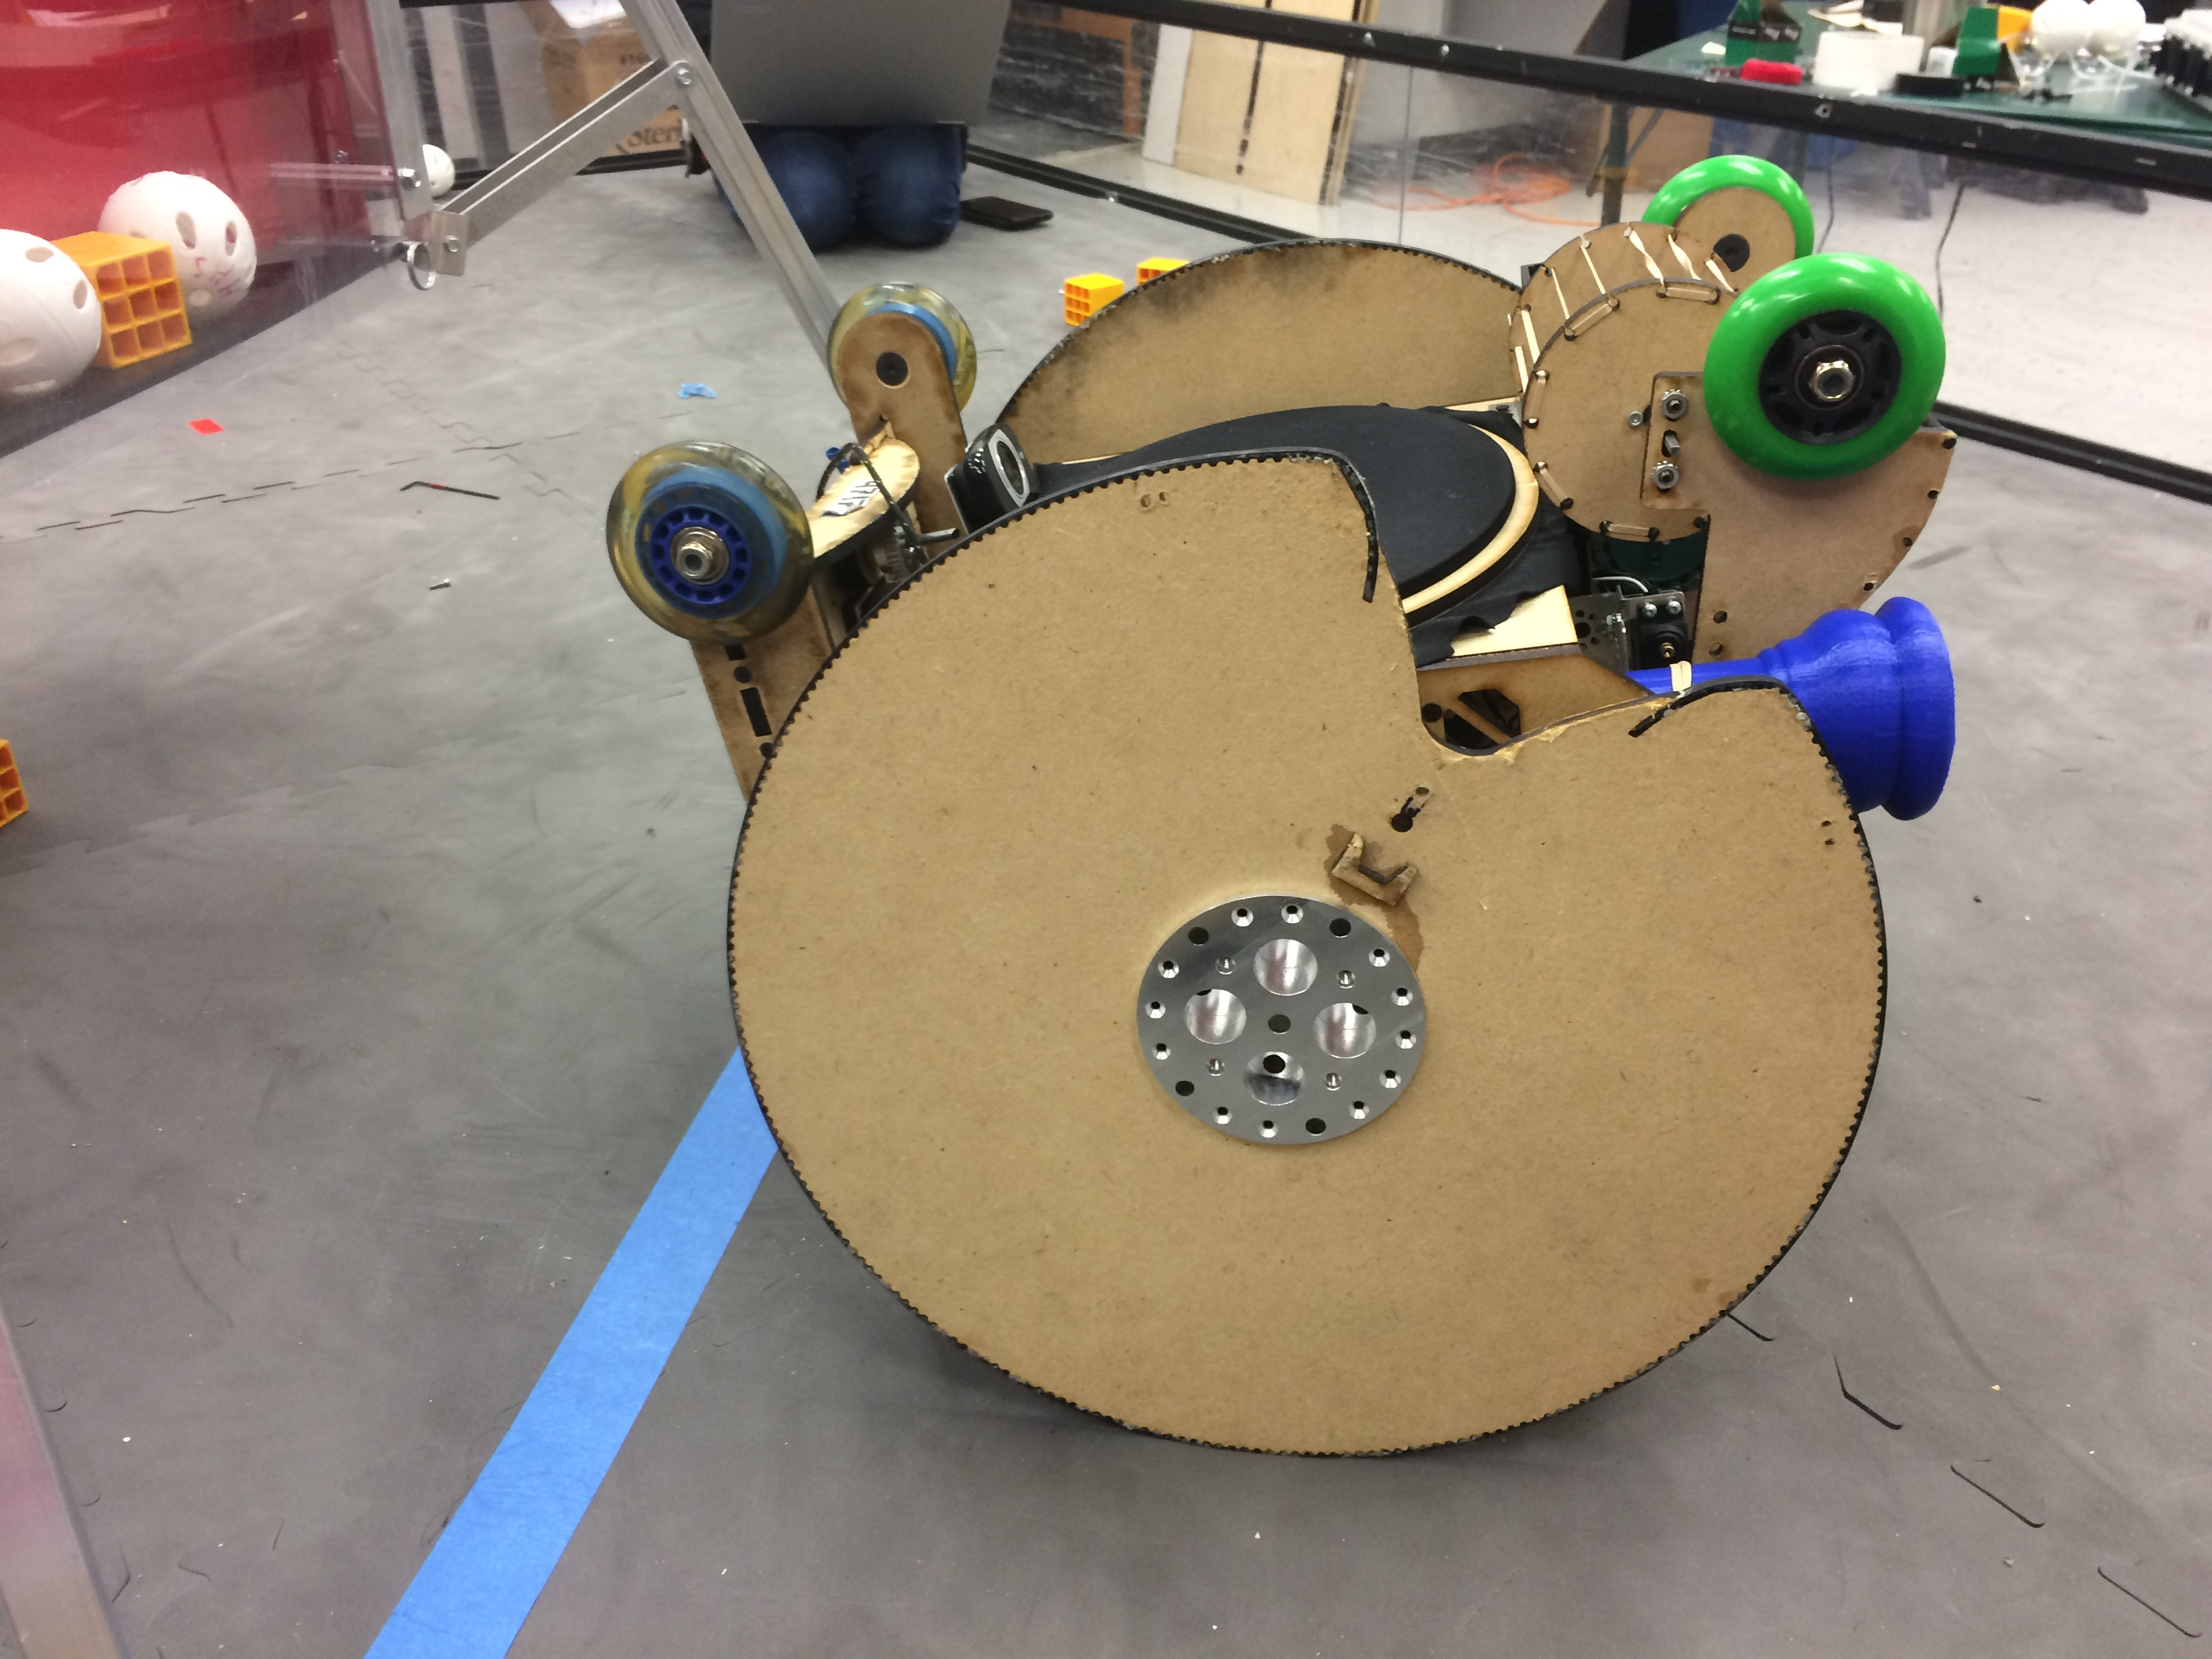
\includegraphics[width= .9\linewidth]{Design_Overview/Zero.JPG} %%zero
\end{minipage}%
\hfill
\begin{minipage}{.32\textwidth}
  \centering
  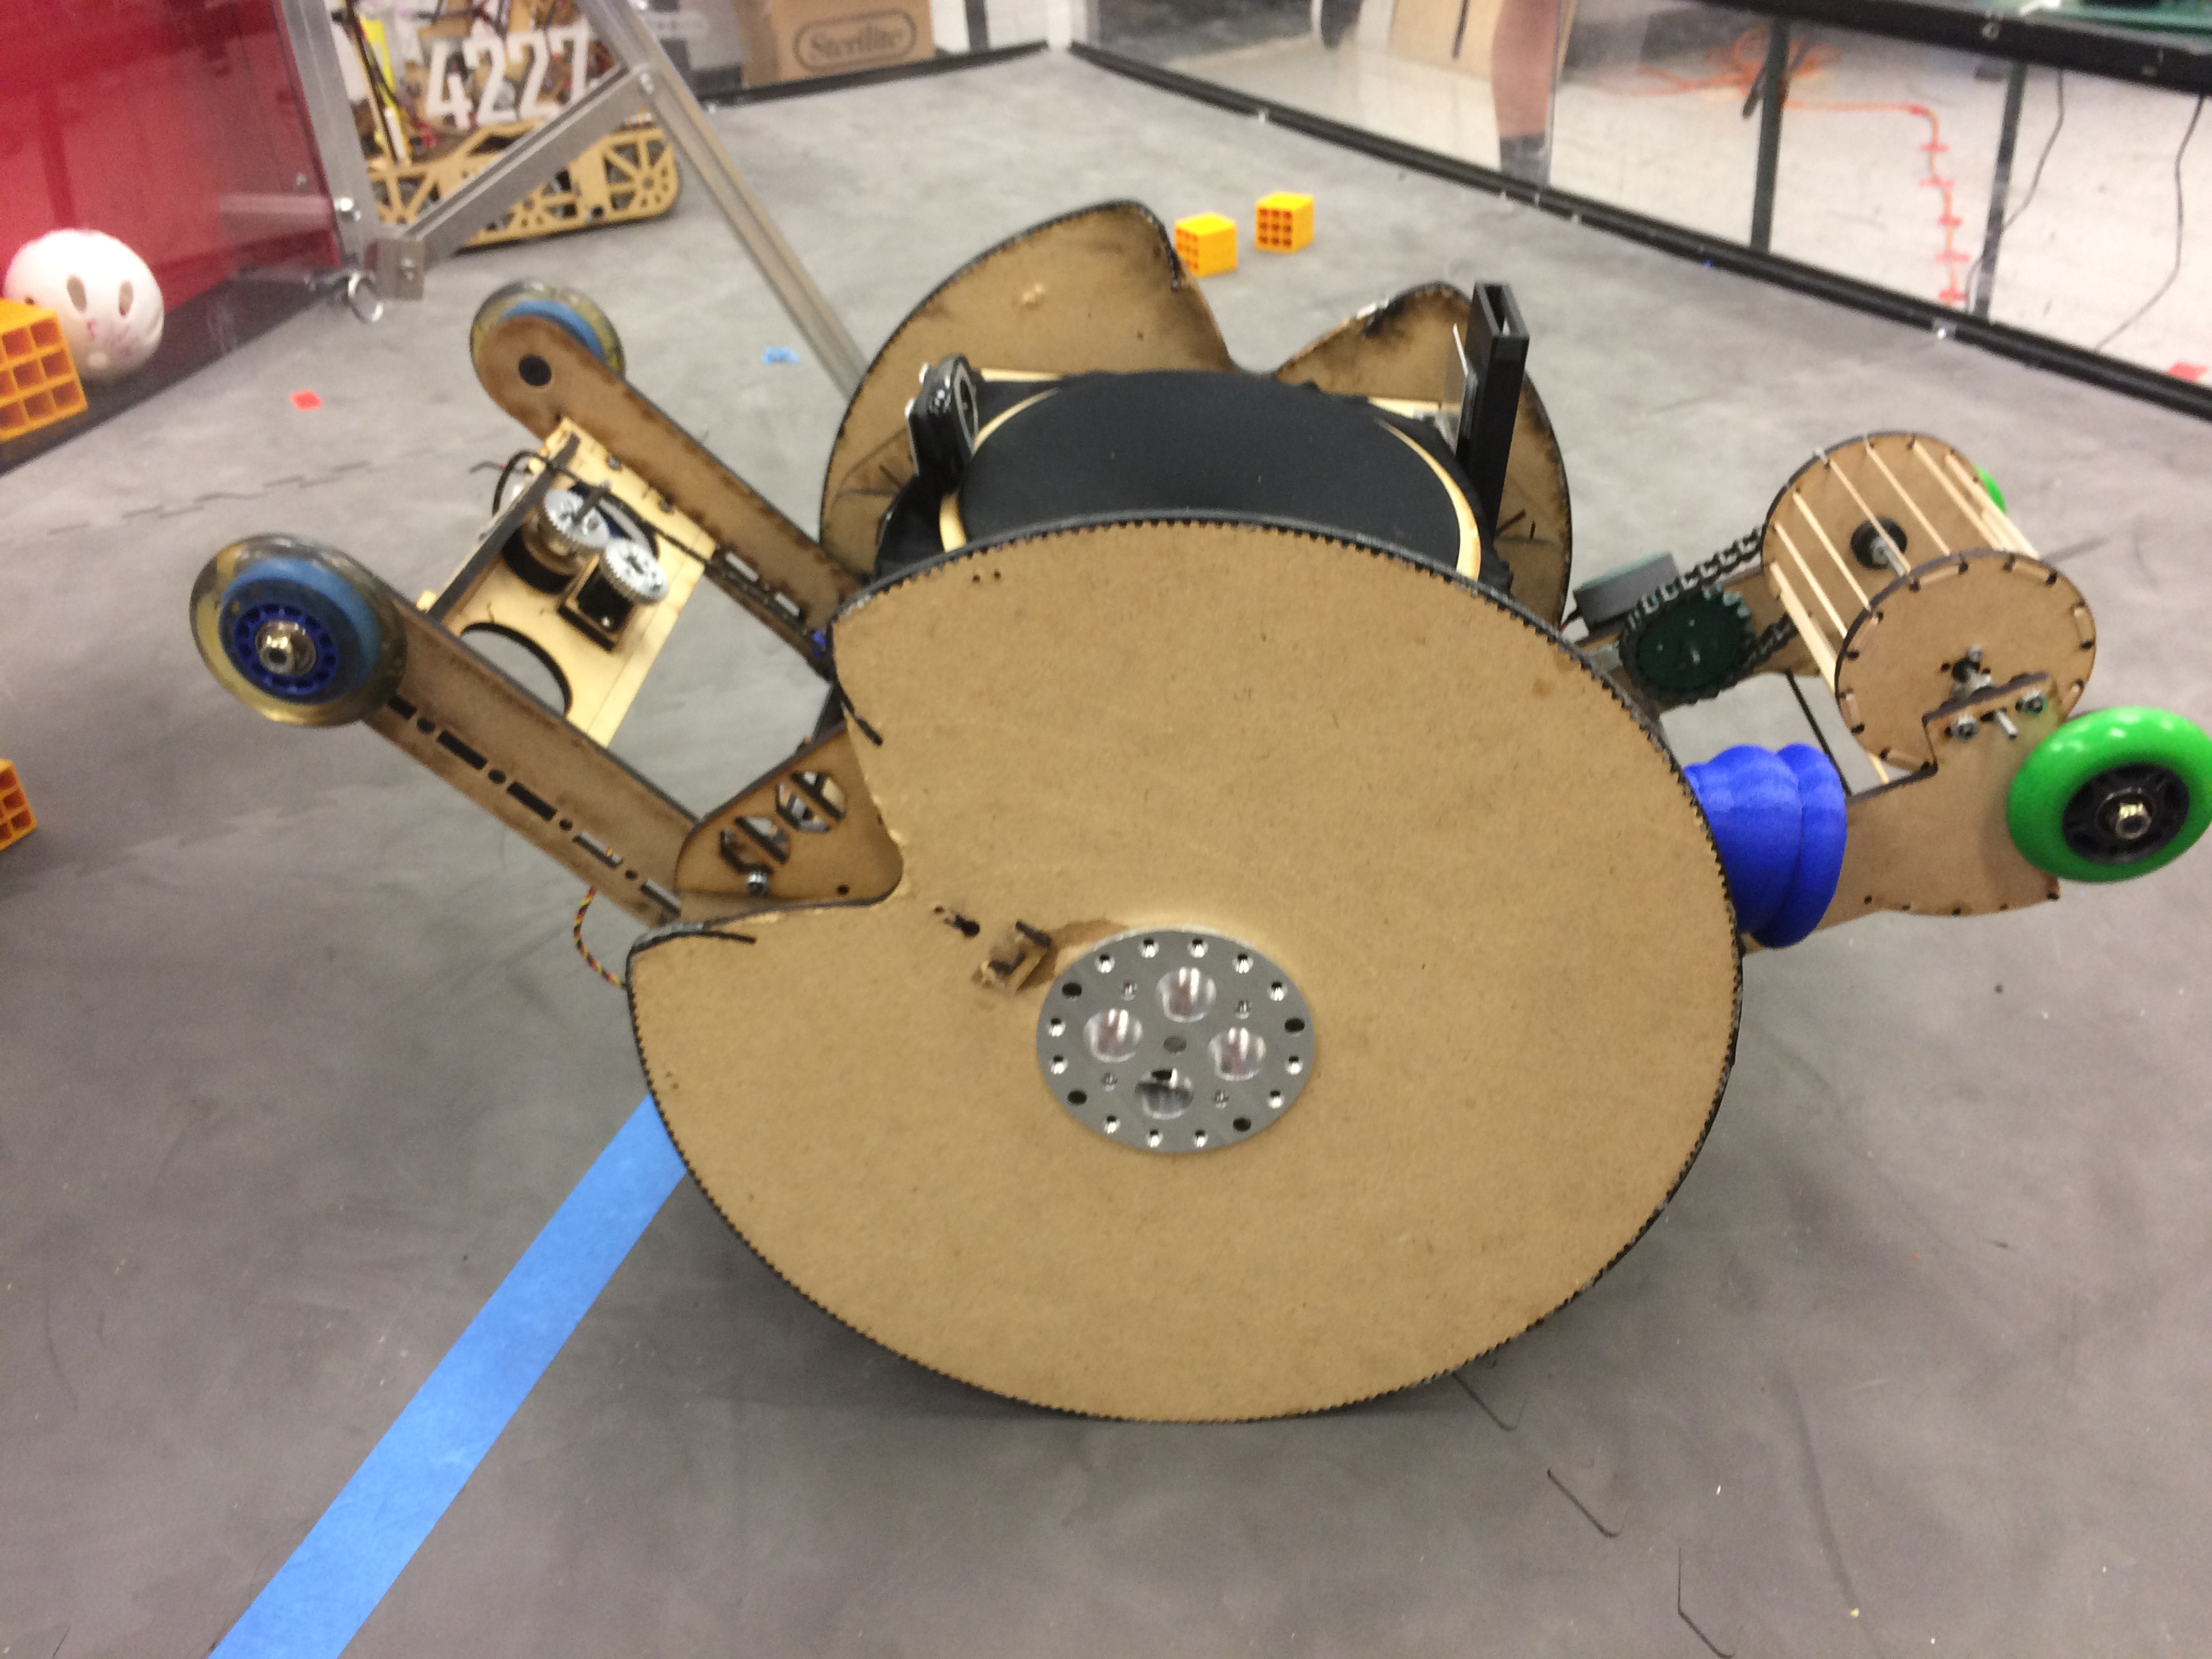
\includegraphics[width= .9\linewidth]{Design_Overview/45.JPG} %%45
\end{minipage}%
  \hfill
\begin{minipage}{.32\textwidth}
  \centering
  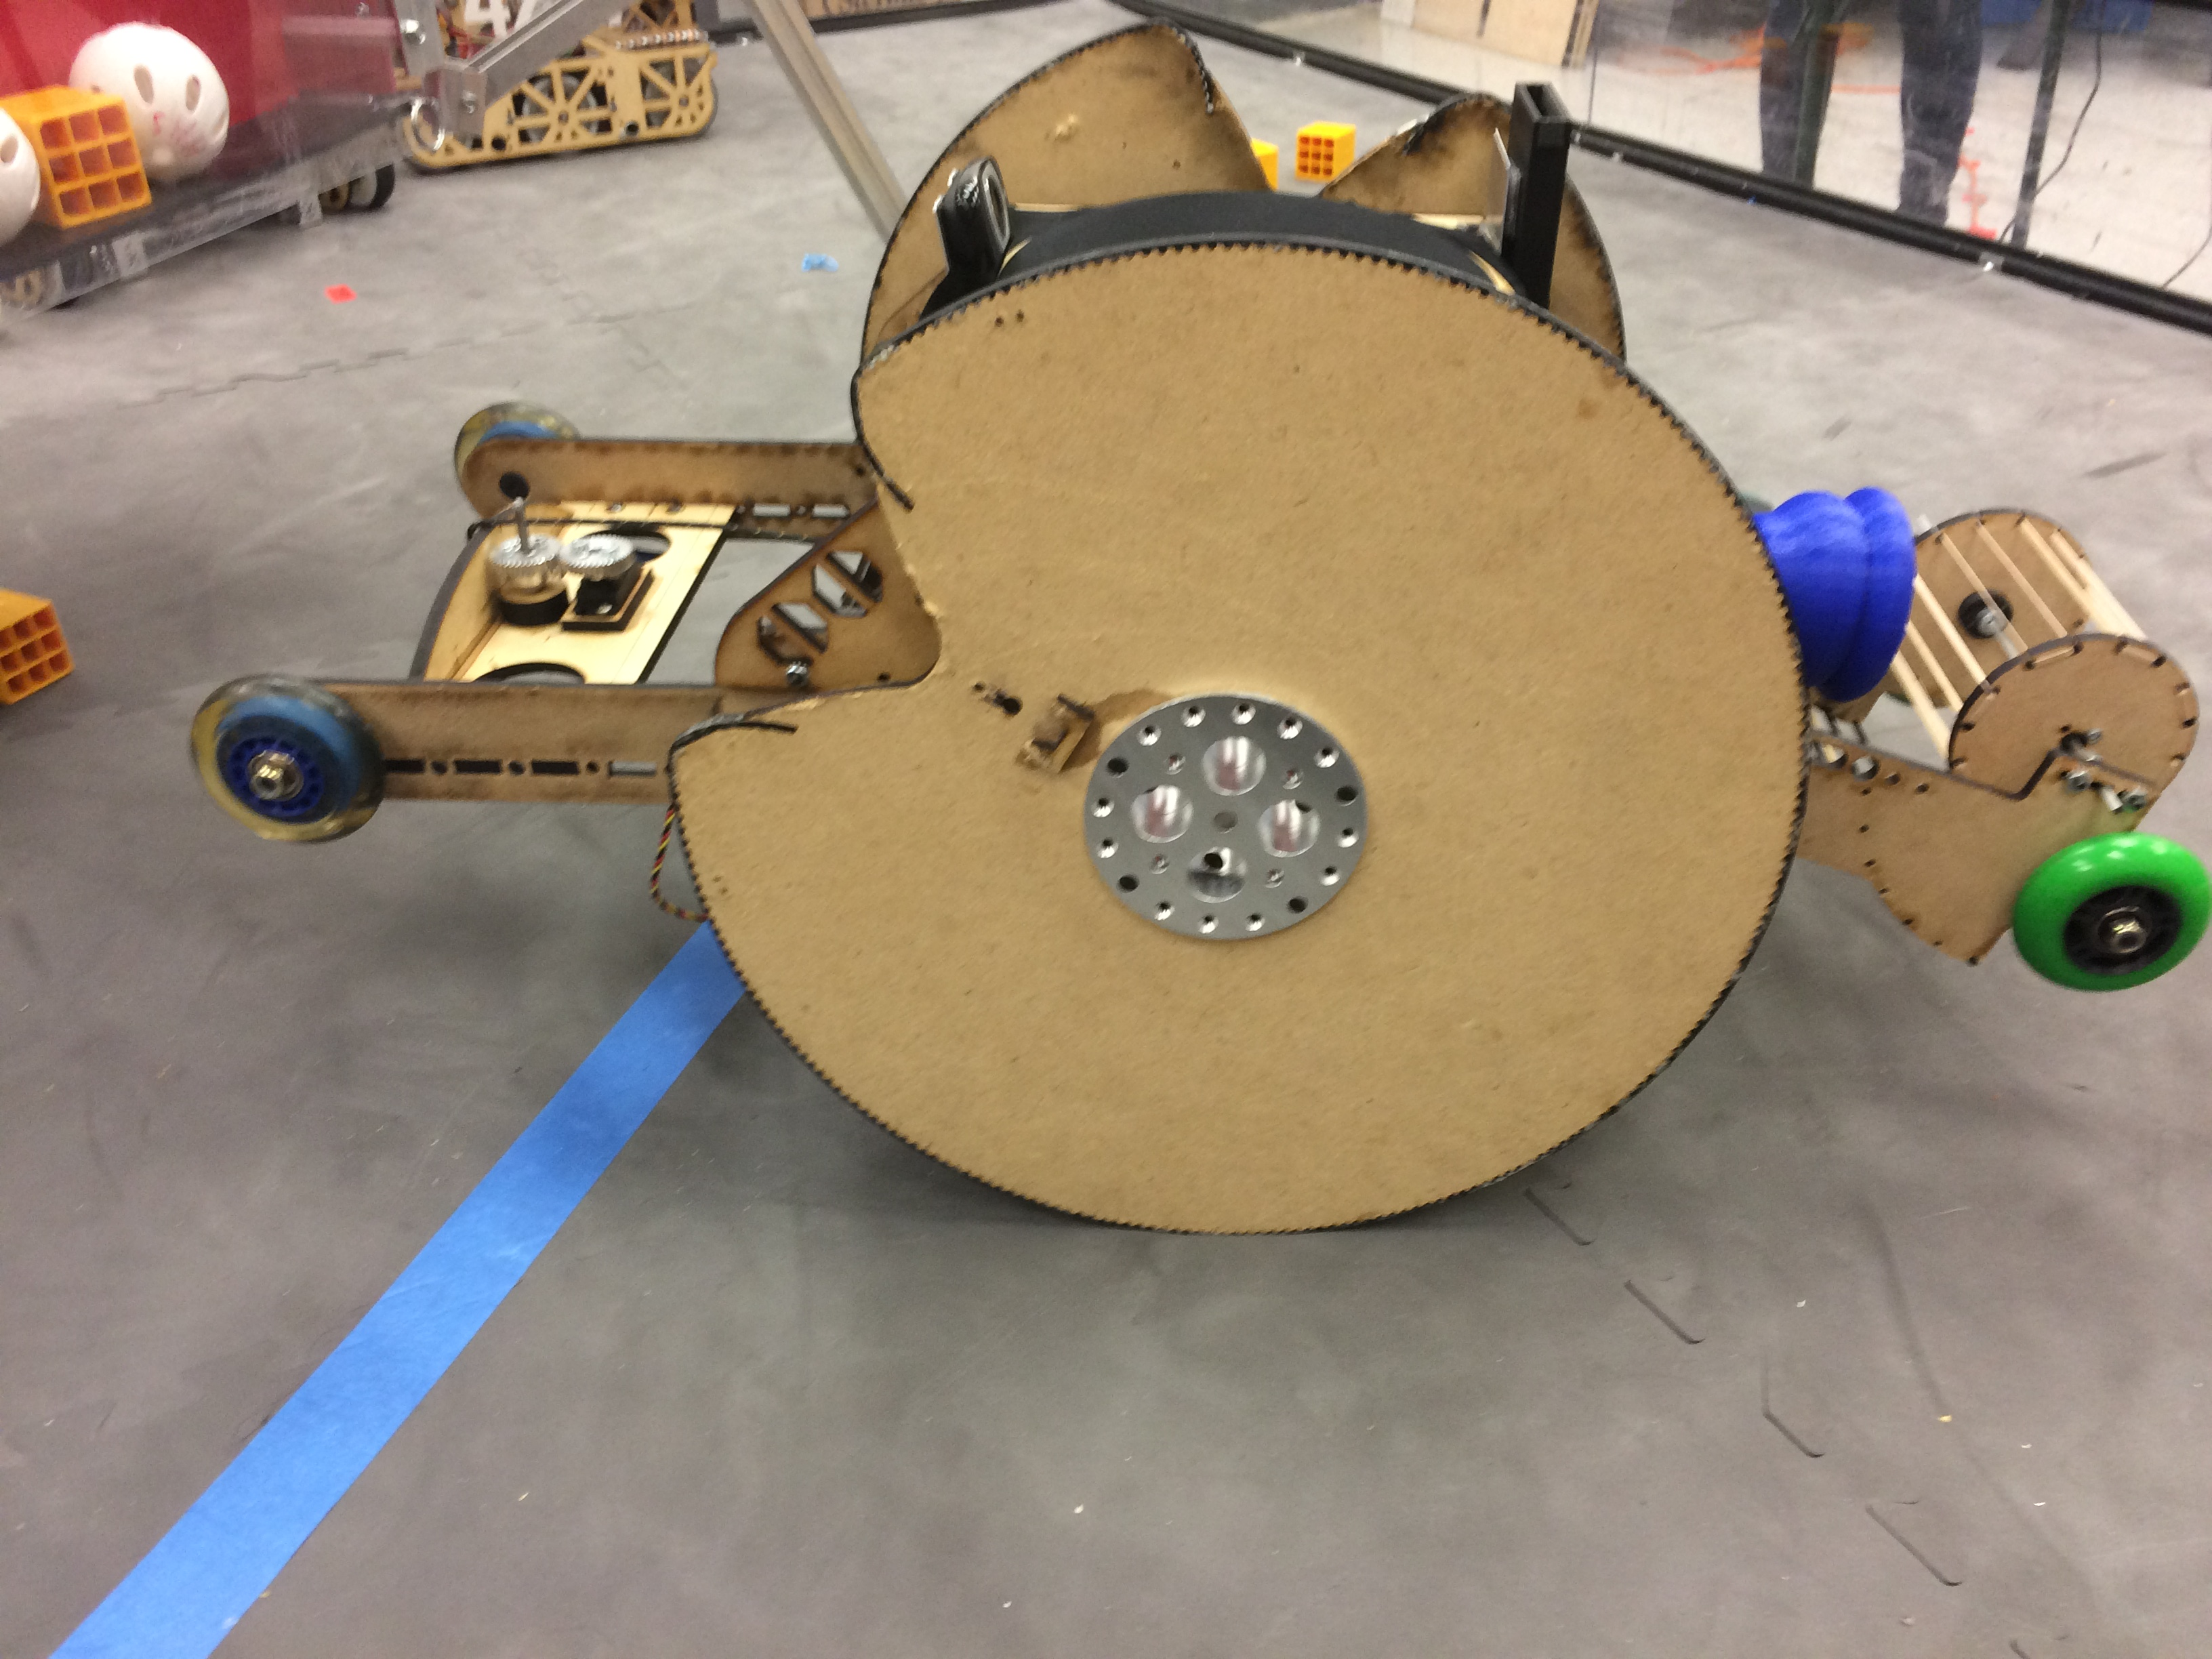
\includegraphics[width= .9\linewidth]{Design_Overview/90.JPG} %%90
\end{minipage}
\end{figure}

\begin{figure}[h!]
\centering
\begin{minipage}{.32\textwidth}
  \centering
  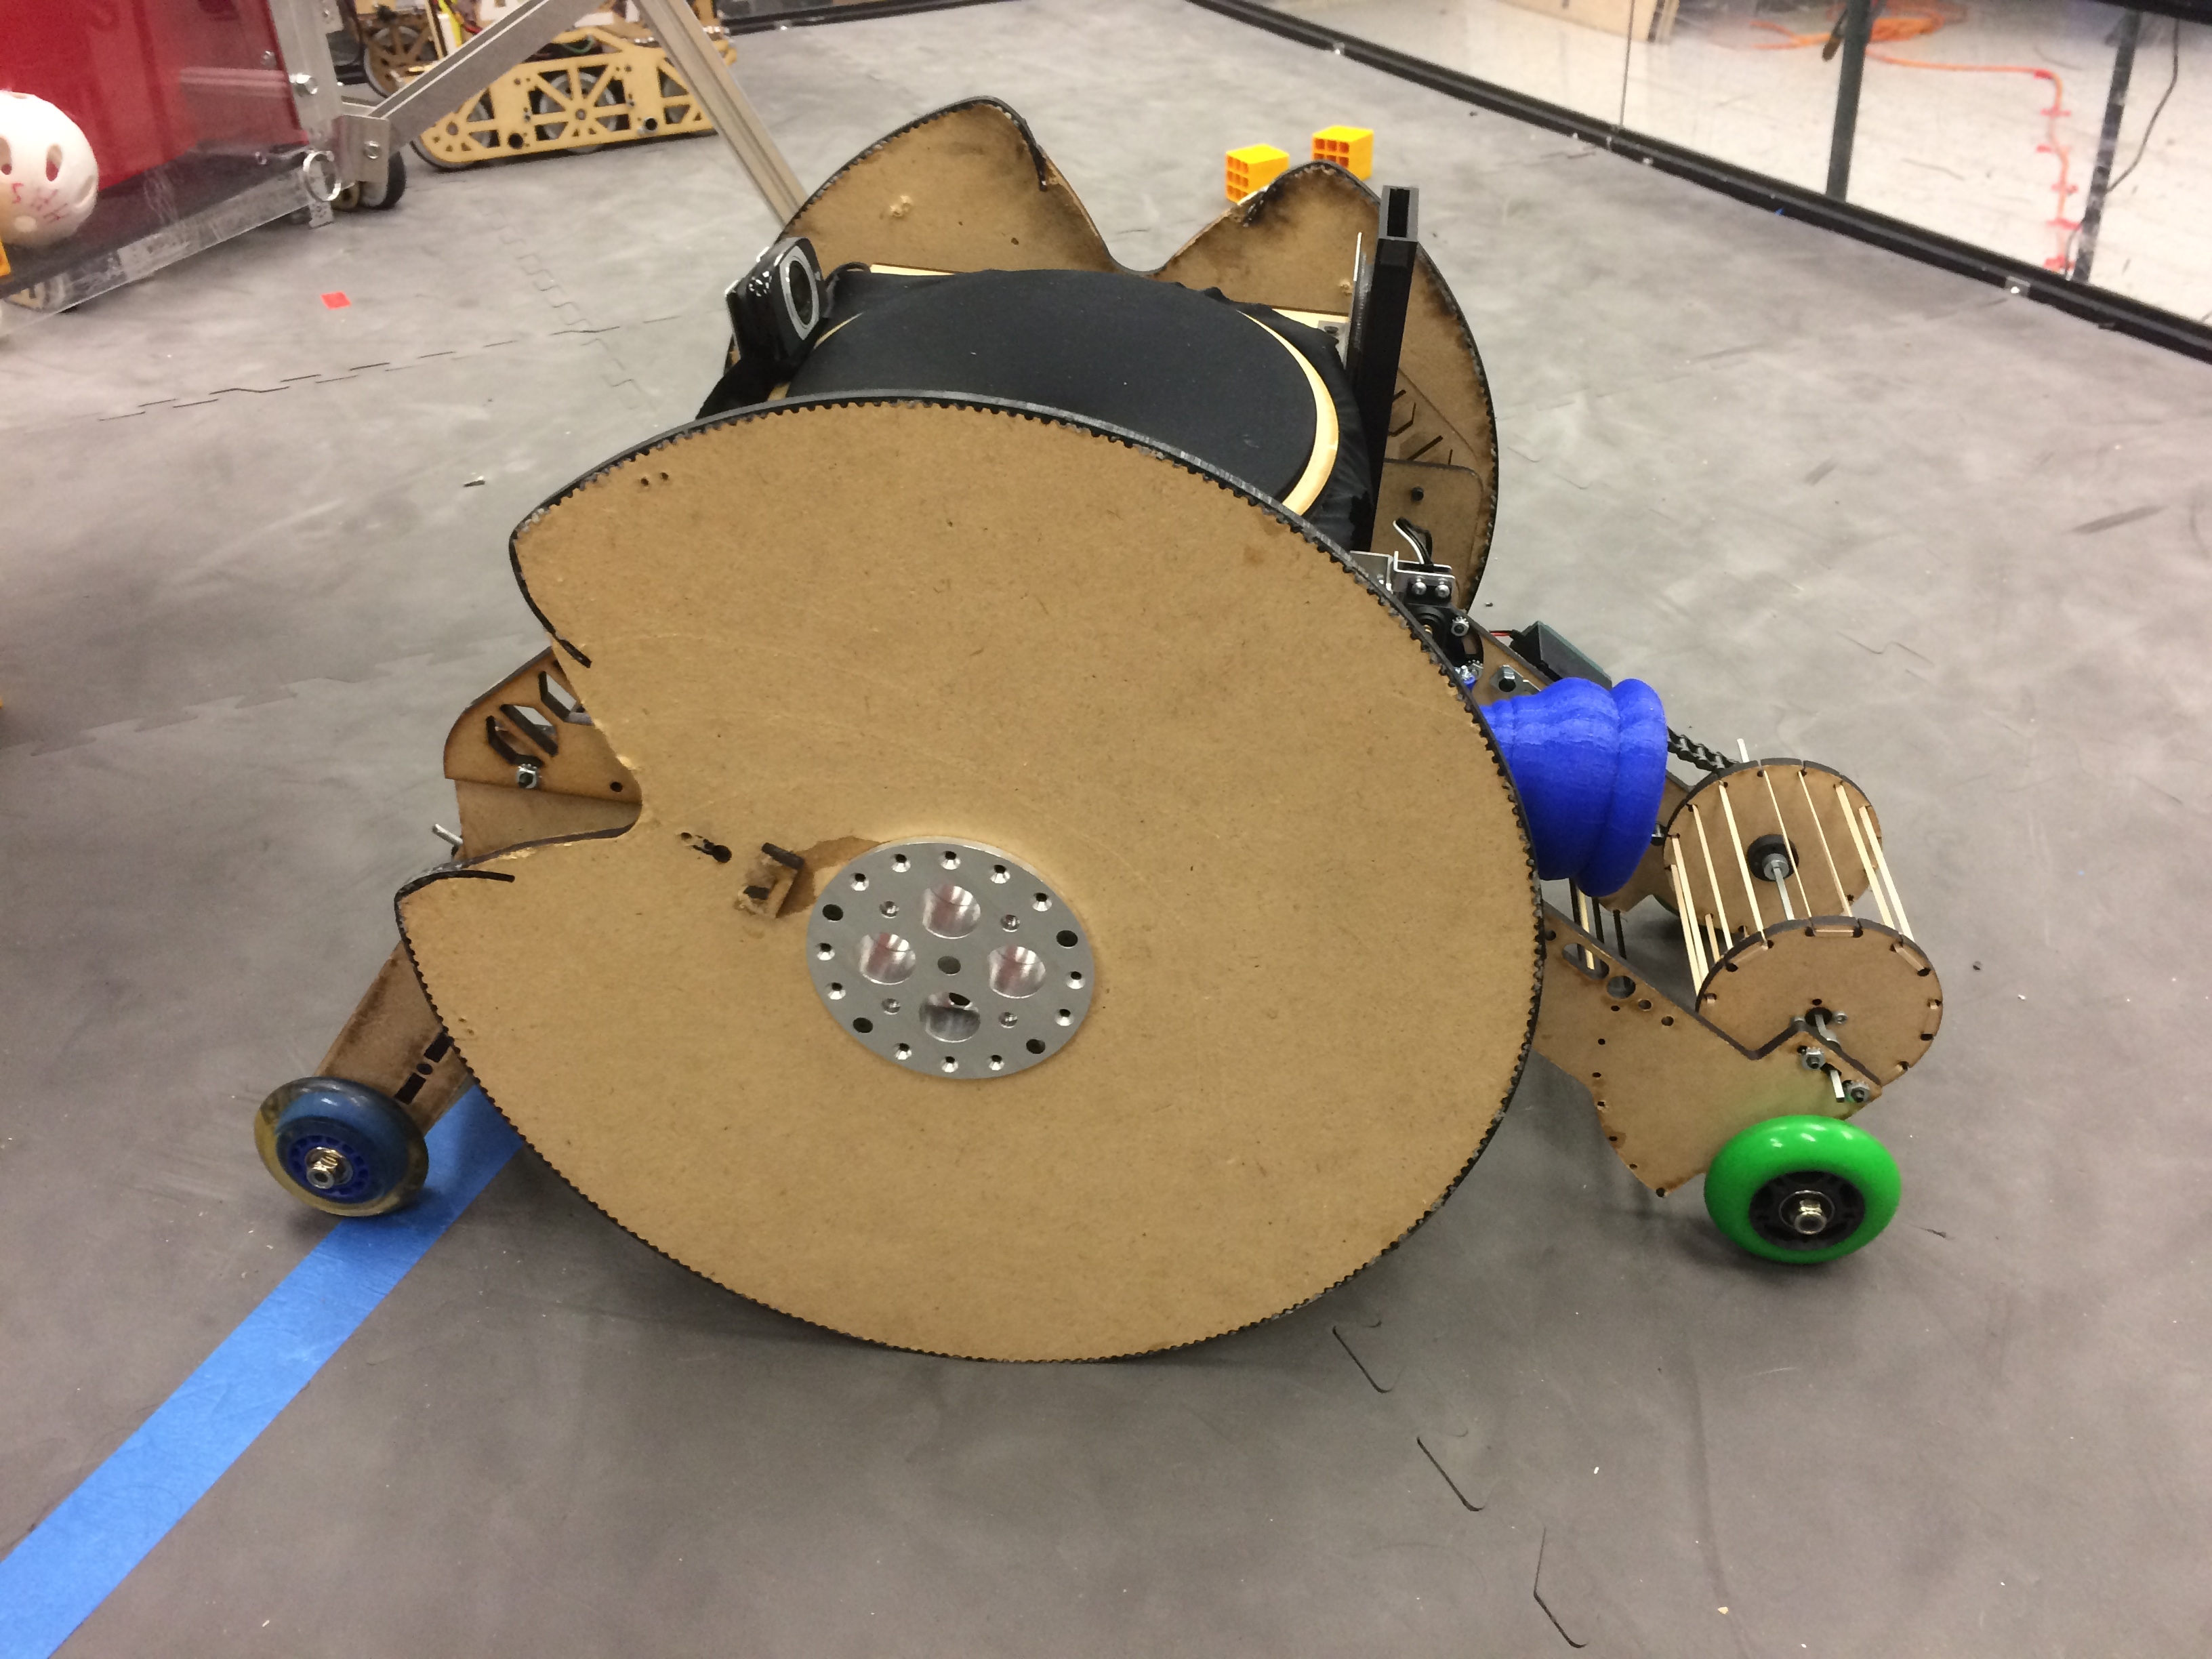
\includegraphics[width= .9\linewidth]{Design_Overview/Natural.JPG} %%natural
\end{minipage}%
\hfill
\begin{minipage}{.32\textwidth}
  \centering
  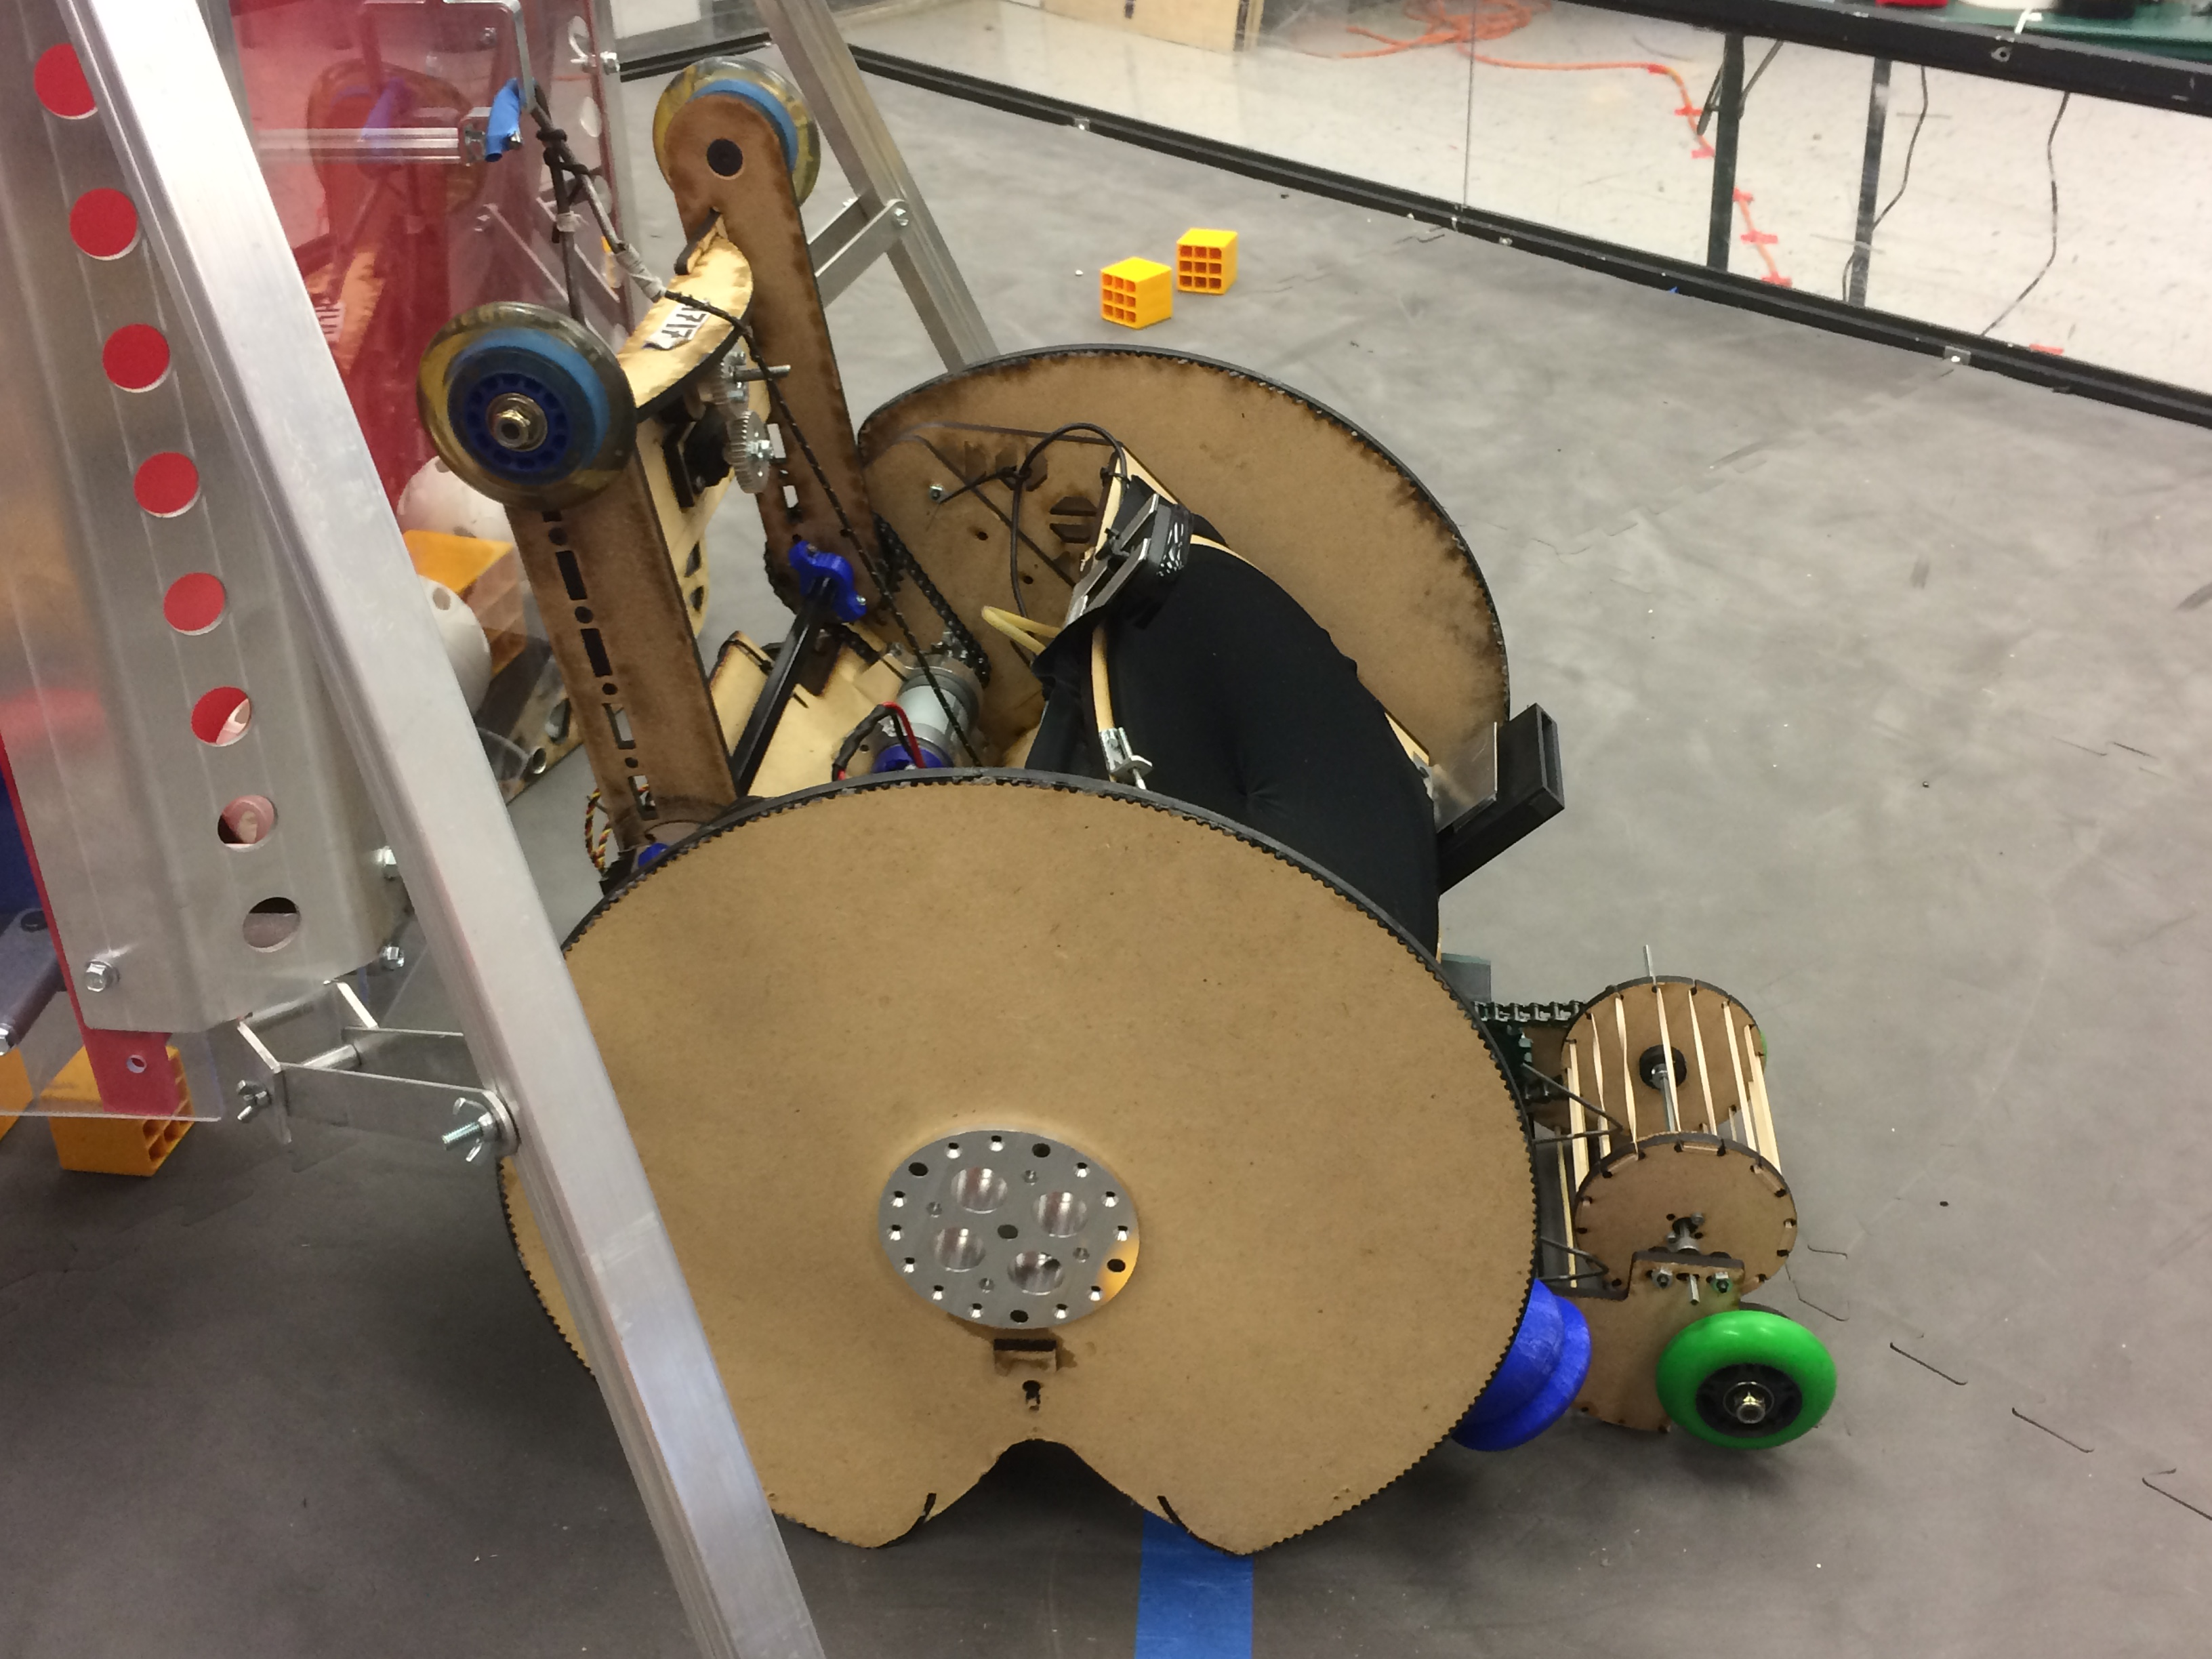
\includegraphics[width= .9\linewidth]{Design_Overview/hang_angle.JPG} %%shooting
\end{minipage}%
  \hfill
\begin{minipage}{.32\textwidth}
  \centering
  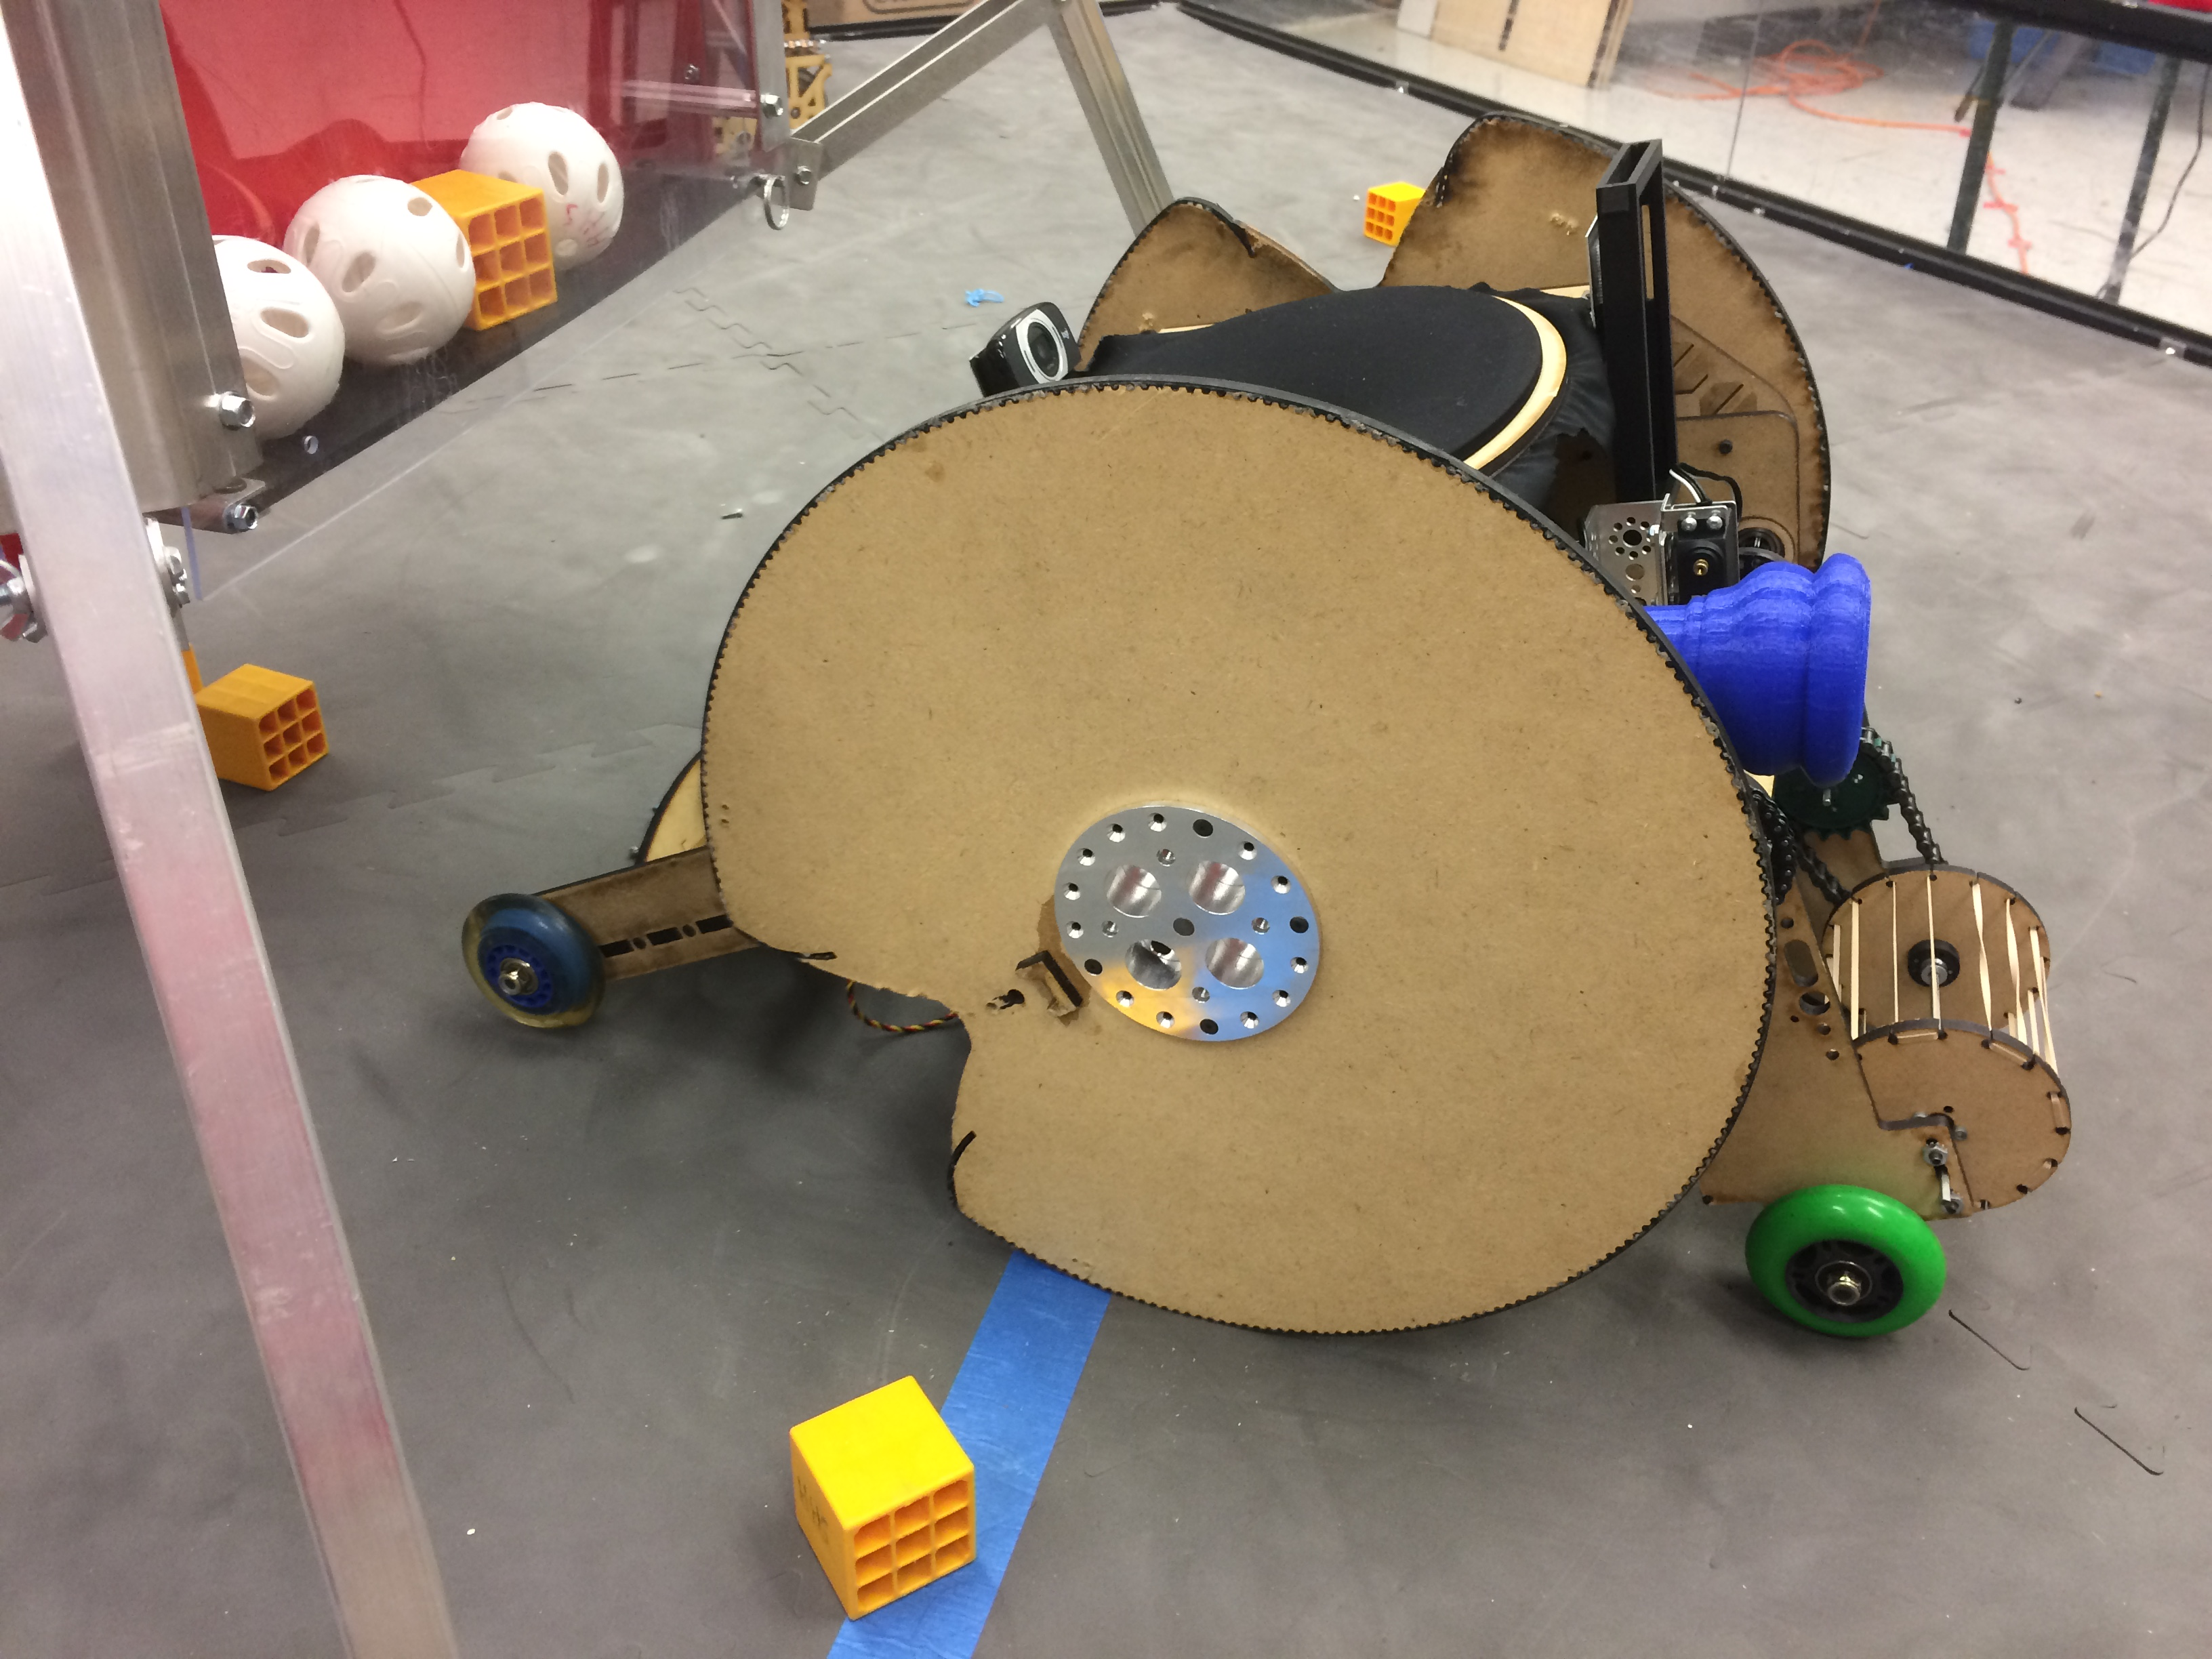
\includegraphics[width= .9\linewidth]{Design_Overview/shooter_angle.JPG} %%hang
\end{minipage}
\end{figure}

\vskip 0.25in
Chassis Stabilization and Level Driving Angles: 
\vskip 0.05in
\textit{
\\The goal is to maintain ground contact of both stabilization arms in order to drive smoothly. 
}

\vskip 0.2in
\begin{equation}
\phi_{front} = \arccos(\frac{sin(\theta) + 6.7 + 6.5}{8.0} - 90 + \theta)
\end{equation}

\begin{equation}
\phi_{back} = \arccos(\frac{-sin(\theta) + 6.7 + 6.5}{8.0} + 90 + \theta)
\end{equation}

\subsection*{Equation Analysis}
\textit{
\\ With the use of one of the angles, we can calculate the angle of the other arm to be stable; Refer to the January 20th entry to learn more about how these equations work, and how we created them. 
}

\interesting{Writing Formulas for Arm Stabilization}{control:2}

\subsection*{Mechanism Accomplishments}
\begin{itemize}
    \item Uniformly stabilize the chassis, maintain ground contact to ensure smooth driving
    \item Set to the prepositioned intake angle to pick up minerals
    \item Set to the prepositioned shooter angle for mineral deposit 
    \item Set to the prepositioned hang angles for the endgame in TeleOp
\end{itemize} 